%%%%%%%%%%%%%%%%%%%%%%%%%%%%%%%%%%%%%%%%%%%%%%%%% PREAMBLE %%%%%%%%%%%%%%%%%%%%%%%%%%%%%%%%%%%%%%%%%%%%%%%%%%

%environment setup
\documentclass[letterpaper,11pt]{article}
\usepackage[square,comma,numbers,sort&compress]{natbib}
\bibliographystyle{ieeetr}
\usepackage{amsmath}
\usepackage{graphicx}
\usepackage{url}
\usepackage{xspace}
\usepackage[left=20mm,top=20mm]{geometry}
\usepackage{hyperref}
\usepackage{lineno}
\renewcommand{\familydefault}{\sfdefault}

%macros
\newcommand{\reffig}[1]{Figure~\ref{#1}}
\newcommand{\refsec}[1]{Section~\ref{#1}}
\newcommand{\refeq}[1]{Equation~\ref{#1}}
\DeclareMathOperator*{\argmax}{arg\,max}
\newcommand{\Tau}{\mathrm{T}}
\newcommand{\Iota}{\mathrm{I}}
\newcommand{\Mu}{\mathrm{M}}
\newcommand{\fmax}{f_{\mathrm{max}}}

%%%%%%%%%%%%%%%%%%%%%%%%%%%%%%%%%%%%%%%%%%%% TITLE AND ABSTRACT %%%%%%%%%%%%%%%%%%%%%%%%%%%%%%%%%%%%%%%%%%%%%

%title
\title{Flatfielding: Correcting Spatial Variations in Microscope High-power Field Illumination}
\author{Maggie Eminizer\\ \url{margaret.eminizer@gmail.com}\\ JHU Astropath Group}
\date{\today}
\begin{document}
\maketitle

%start numbering lines
\linenumbers

%abstract
\abstract{This note details a method for correcting systematic variations in the illumination of multiplexed immunofluorescence microscopy images. The variations are measured using regions of image layers that are free of empty background as determined using a thresholding and masking procedure. The illumination flux observed in these regions is averaged over a large number of images, and the resulting variation pattern is smoothed to retain only the large-scale effects. The spatially-dependent corrections are defined as the ratios of these average flux patterns to their mean values in each image layer. The corrections are measured and the effects of their application are characterized using a set of 45,384 melanoma tissue images collected at the Johns Hopkins Hospital using an Akoya Biosciences Vectra 3.0 digital microscope. It is shown that the illumination of the tissue depicted in these images initially varies with an average standard deviation of 3.64\% relative flux in systematic patterns for each image layer, and that applying the corrections reduces the variation to an average standard deviation of 0.37\% relative flux in more random patterns.}

%%%%%%%%%%%%%%%%%%%%%%%%%%%%%%%%%%%%%%%%%%% INTRODUCTION SECTION %%%%%%%%%%%%%%%%%%%%%%%%%%%%%%%%%%%%%%%%%%%%
\section{Introduction}
\label{sec:introduction}

The Astropath group's work in quantifying patient outcomes from cancer immunotherapies is largely driven by analysis of multiplexed immunofluorescence microscopy images. As the group maintains focus on scaling up to curate and analyze large datasets representing multiple types of cancers contributed by a variety of primary sources or collaborators, a major push continues to be performing as much of that image analysis as possible in an automated fashion. It is therefore imperative that the image data themselves are of a very high quality, corrected for subtle effects that may adversely impact how individual images are related to one another to represent an entire microscope slide, or how the contents of those slides may be identified by automated algorithms as cells expressing certain immunofluorescence markers of interest. This note discusses a method developed to perform a low-level initial correction to the illumination of raw microscope images, and details the effect of applying this correction to an example dataset. 

%%%%%%%%%%% Flatfielding in general subsection
\subsection{Flatfielding in general}
\label{ssec:flatfielding_in_general}

The microscopes used in the Astropath group's analyses all collect light reflected off a sample illuminated by an external light source. Nonuniformities in the microscope optical path and other aspects of the methods by which slides are illuminated inherently introduce a type of systematic noise that appears as variations in the amount of illumination flux recorded at certain points in each collected image. These effects, which make some image regions brighter on average than others, tend to be especially pronounced at the edges of images, and are known interchangeably by terms including ``intensity nonuniformity,'' ``uneven shading,'' ``vignetting,'' or just ``illumination variation'' \cite{doi:10.1111/jmi.12178}. The term ``flat field correction'' (or ``flatfielding'') refers to procedures designed to minimize these systematic illumination variations as they appear in high-power field (HPF) fluorescence microscopy images. 

Although the effects of uneven illumination may barely be noticeable within single images or during qualitative image analysis, they become much more problematic when large groups of images are analyzed, or when highly quantitative analyses that depend entirely on pixel illumination flux content are performed. The Astropath group's procedure for aligning and stitching individual HPF images together to represent a single high-magnification image of an entire slide is an example of such a flux-dependent quantitative analysis that would be adversely affected by certain regions of HPF images being brighter in general than others \cite{Heshy}. Other methods currently in development for automated segmentation of cells and quantitative pathology will also likewise depend on reliable measurements of illumination flux.

Methods for correction of the type of illumination variation in question have long existed, and are often built into digital microscopy image analysis platforms like CellProfiler \cite{Carpenter2006}, or even directly into automated microscope imaging procedures. These correction methods can generally be separated into the two categories of ``a-priori,'' referring to corrections derived from calibration materials imaged through the same methods as the samples of interest, and ``a-posteriori,'' referring to corrections determined only from the images of interest themselves \cite{18770694}. A-priori methods are particularly limited in effectiveness for applications in digital, high-throughput, fluorescence microscopy because they require time and infrastructue investment in additional imaging of reference samples; the reference samples themselves can be nontrivial to prepare such that they fluoresce identically to biological samples; and because additional digital noise beyond optical effects may impact illumination variation \cite{doi:10.1111/jmi.12178}.

A-posteriori methods have therefore been developed using a variety of approaches, including modeling additive and multiplicative noise components and fitting the model to data by minimizing the entropy of the corrected image \cite{PMID:10692132} or filtering images for low-frequency illumination variations and correcting the pattern observed at this frequency \cite{Leong619}. Authors have also made important distinctions between illumination variation affecting slides as a whole as opposed to just the tissue or cells within an image \cite{Carpenter2006}. The method the Astropath group has developed is a-posteriori by design, and uses large samples of images of interest to measure and correct large-scale illumination variation. The advantages of this approach are that no additional imaging of calibration samples is necessary, and that the measured corrections are unbiased to regions of images that show only background and not the tissue used for pathological analysis.

%%%%%%%%%%% Work already performed subsection
\subsection{Work already performed}
\label{ssec:work_already_performed}

The Astropath group's investigations of systematic illumination variation effects began in 2017, when substantial effects were noticed in Tissue Microarray (TMA) and deep tissue microscope images. In the first version of the work, documented in \cite{Alex_flatfielding_1}, an a-priori method was used to model the effects, wherein a slide of light diffusing material was imaged using identical methods to the slides of interest. The composite image layers, unmixed from their initial component layers, were normalized by their mean illumination flux, resulting in the pattern shown on the upper left-hand side of \reffig{fig:first_flatfielding} for the DAPI layer of the unmixed image. This pattern was fit with a two-dimensional, second degree polynomial function, shown on the upper right-hand side of \reffig{fig:first_flatfielding}. The flux at each pixel in the first layer of the full individual component IM3 image was then divided by the associated value of the function fitted to the unmixed DAPI layer, and a resulting decrease in the systematic illumination variation was observed, as shown in the lower plot in \reffig{fig:first_flatfielding}. Similar methods using a third-degree polynomial fit were applied to the other layers of the unmixed images, as well as the individual component IM3 layers, with varying results. It was concluded that a polynomial fit was likely insufficient to describe the illumination variations in all image layers.

\begin{figure}[!ht]
\centering
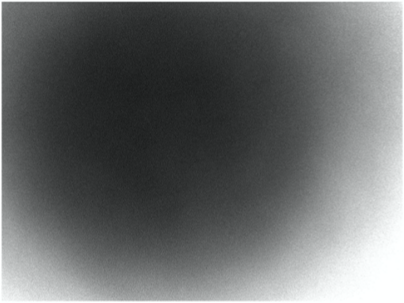
\includegraphics[width=0.45\textwidth]{images/introduction/first_unmixed_DAPI_meanimage}
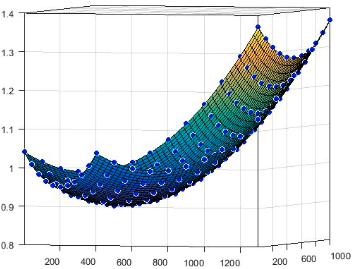
\includegraphics[width=0.45\textwidth]{images/introduction/first_DAPI_meanimage_polynomial_fit}
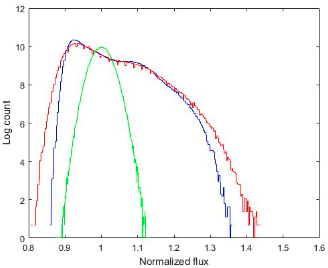
\includegraphics[width=0.45\textwidth]{images/introduction/first_DAPI_meanimage_corrected_flux}
\caption{\footnotesize Upper left: Illumination flux pattern observed in the unmixed DAPI layer of an imaged light diffuser. Upper right: two-dimensional, second-degree polynomial fitted to the mean-normalized flux pattern pictured in the upper left figure. Lower: Histogram of log pixel counts vs. mean-normalized flux for the light diffuser image's unmixed DAPI layer (in red), first component IM3 layer (in blue), and first component IM3 layer after pixelwise division by the polynomial shown in the upper right plot (in green); the applied correction has reduced the systematic illumination variation to more Gaussian noise. Figures from \cite{Alex_flatfielding_1}.}
\label{fig:first_flatfielding}
\end{figure}

After these initial investigations, the decision was made to correct illumination variations in images in the raw IM3 component layers rather than in the unmixed composite image layers, and a new a-posteriori method was devloped to model the effects, as documented in \cite{Alex_flatfielding_2}. In this method, the flatfielding corrections were determined by making a single, multi-layer, average raw image from a set of 7,358 HPFs, smoothing the layers of the mean image with a Gaussian filter of standard deviation $\sigma=100$ pixels to retain only the large-scale pattern, and dividing this smoothed mean image by the mean average flux value layer-by-layer so that the corrections did not change the overall illumination of each image layer. It was found that this method resulted in consistent illumination variation patterns, shown in \reffig{fig:second_flatfielding}, correlated within layers contributing to the same broadband filter region (raw layers 1-9, 10-18, 19-25, 26-32, and 33-35 for the DAPI, FITC, Cy3, Texas Red, and Cy5 unmixed spectral components, respectively).

\begin{figure}[!ht]
\centering
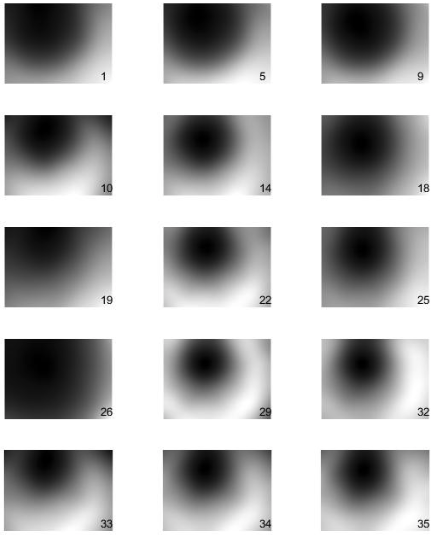
\includegraphics[width=0.9\textwidth]{images/introduction/second_flatfield_image_layers}
\caption{\footnotesize Selected layers of the flatfield image from \cite{Alex_flatfielding_2}, stretched from minimum to maximum mean-normalized flux, in the first, middle, and last layer of each broadband filter region as labeled. The patterns are fairly consistent between each broadband filter break. Layer 26, the first layer in the Texas Red region, was not brightly illuminated for the melanoma tissue samples used, and represents an outlier in this and other investigations.}
\label{fig:second_flatfielding}
\end{figure}

After using this new model for some time to correct HPF illumination, it was discovered \cite{Ben_flatfielding_1} that the algorithm implemented in the inForm software package \cite{Kramer2018} used to phenotype cells for pathology was over-identifying cells of a certain type in some more recently-collected samples, in a pattern similar to that of the original flatfield correction images. Updated flatfield correction models were developed using the same averaging, smoothing, and normalizing method as in \cite{Alex_flatfielding_2} for different subsets of the data separated by time of collection (or ``batch''), and it was discovered that changing the lightbulb in the microscope between batches had a significant effect on the pattern of illumination variation, as shown in \reffig{fig:third_flatfielding}. 

\begin{figure}[!ht]
\centering
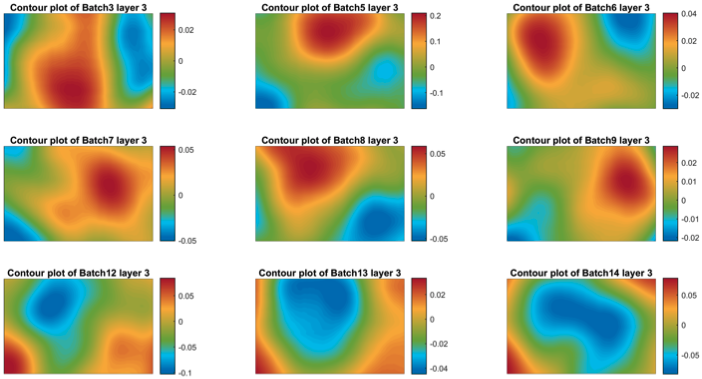
\includegraphics[width=0.9\textwidth]{images/introduction/third_flatfield_differences}
\caption{\footnotesize Differences in the third unmixed image layer between the normalized mean images computed independently for each batch and the original flatfield correction image measured in \cite{Alex_flatfielding_2} using a subset of the Batch3 data. These images showed that the illumination variations changed between batches, and especially for batches 12 and 13-14, before the collection of which the lightbulb in the microscope was replaced. Figures from \cite{Ben_flatfielding_1}.}
\label{fig:third_flatfielding}
\end{figure}

At this point the decision was made to measure and correct for the illumination variations independently for each batch of images collected. The work documented in \cite{Ben_flatfielding_1} also gave the first look at the illumination variations in samples collected with the Vectra Polaris imaging system as opposed to the Vectra 3.0 digital microscope, showing that the overall amount of variation was less for the Vectra Polaris, and the patterns were different in shape, likely due to the Vectra Polaris using an LED array rather than a lightbulb for slide illumination. This comparison was made in greater detail in \cite{Ben_flatfielding_2} where two component-layer mean image models were computed from sets of 10,000 HPFs collected with the Vectra 3.0 and Vectra Polaris microscopes. The corrections were applied to sets of 10,000 independent HPF datasets from each microscope, and the uncorrected and corrected images were unmixed using inForm. It was discovered that applying the flatfield corrections greatly reduced the overall illumination variation in the average unmixed images for both the Vectra 3.0 and Vectra Polaris microscopes, as shown in \reffig{fig:fourth_flatfielding}. To date this type of model of the average of large sets of images is used for correcting illumination variation before unmixing.

\begin{figure}[!ht]
\centering
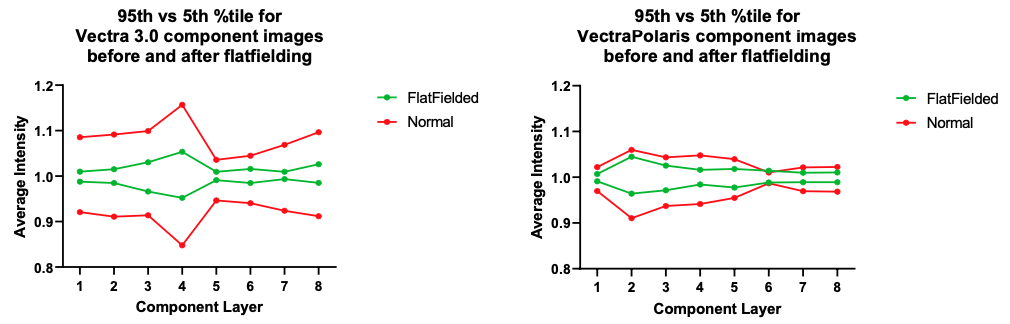
\includegraphics[width=0.9\textwidth]{images/introduction/fourth_flatfield_impact}
\caption{\footnotesize 5th and 95th percentile illumination flux relative to the layer mean in smoothed, unmixed average images before and after application of flatfielding corrections for data collected with the Vectra 3.0 and Vectra Polaris microscopes. The flatfielding corrections and the averages of the images to which they were applied were determined using independent sets of 10,000 HPFs each. Applying flatfield corrections of this type of smoothed, normalized, mean image layers reduced the overall illumination variation observed for images from both microscopes. Figures from \cite{Ben_flatfielding_1}.}
\label{fig:fourth_flatfielding}
\end{figure}

%%%%%%%%%%% This work subsection
\subsection{This work}
\label{ssec:this_work}

It is the goal of the work documented in this note to provide the most detailed and highest quality measurements of the illumination variation and associated flatfield corrections yet made by the Astropath group. To this end, an additional step has been implemented in the flatfielding procedure to only average over regions of images that show tissue, since the inclusion of empty background regions may bias measurements away from noise specifically affecting the tissue used for quantitative clinical pathology further down the line. A secondary goal of this work is to re-implement the analysis pipeline in python, an open-source programming language, and to develop a single software package that is easy to use and able to scale up to even higher throughput without complicating analysis or prohibitively increasing runtime.

The findings presented in this note were prepared using a total set of 45,384 HPFs from 46 individual slides of melanoma tissue samples collected with the Vectra 3.0 digital microscope. The raw images all had 35 layers, and each layer had a length of 1,344 pixels and a width of 1,004 pixels. The set of images was randomly divided into two subsamples of 22,692 HPFs each; one subsample was used to produce the flatfield corrections, and the other subsample was used to measure the illumination variation before and after application of the flatfield corrections.

\refsec{sec:image_masking} below discusses the methods used to identify tissue and mask background out of the HPFs of each sample. \refsec{sec:measuring_flatfield_corrections} explains how images were stacked, averaged, and smoothed to produce measurements of the flatfield corrections. \refsec{sec:results} shows the resulting flatfield image layers and details how their application reduced the illumination variation measured in the independent subsample. A brief summary is presented in \refsec{sec:summary}.

%%%%%%%%%%%%%%%%%%%%%%%%%%%%%%%%%%%%%%%%%%% IMAGE MASKING SECTION %%%%%%%%%%%%%%%%%%%%%%%%%%%%%%%%%%%%%%%%%%%
\section{Image Masking}
\label{sec:image_masking}

One of the main goals of this work is to ignore as much empty background as possible in the images used to measure the flatfield corrections. The background portions of the images are inherently illuminated differently than the fluorescent tissue, so including background may bias measurements away from what would be observed for the tissue alone. The separation of tissue from background is achieved using a masking procedure.

%%%%%%%%%%% Determining background flux thresholds subsection
\subsection{Determining background flux thresholds}
\label{ssec:determining_background_flux_thresholds}

The first step in masking background out of images is to find flux thresholds above which a pixel is more likely to represent bright tissue than dim background. Because of differences in staining, illumination, exposure time, and fluorescence, these background flux thresholds are measured independently for each layer of each sample. A clear threshold is easiest to determine when a given image layer shows both some tissue and some background, which is often not the case in the bulk of the tissue samples, so thresholds are determined using HPFs located on the edges of the tissue in each sample. The locations of these edge HPFs are shown in \reffig{fig:edge_HPFs} for a few examples. A set of optimal flux thresholds per layer is found for each of these images independently, and the final optimal layer thresholds for each sample are the means of these individual measurements.

\begin{figure}[!ht]
\centering
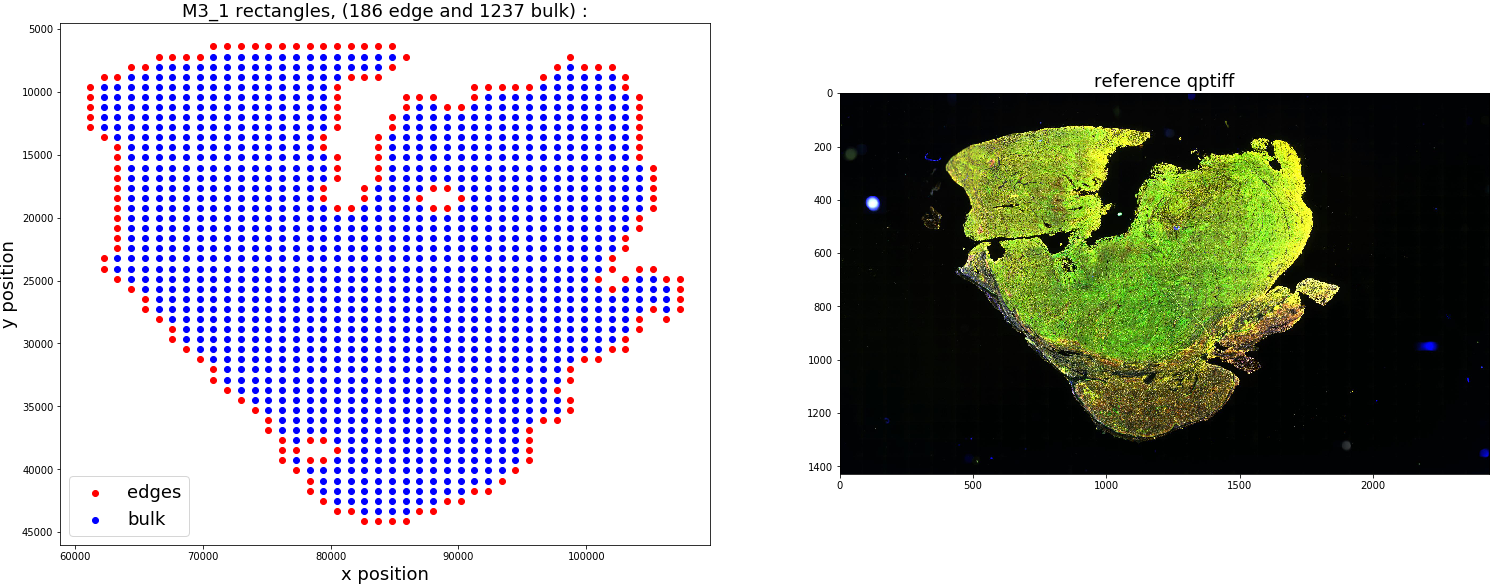
\includegraphics[width=0.95\textwidth]{images/masking/rectangle_locations_M3_1}
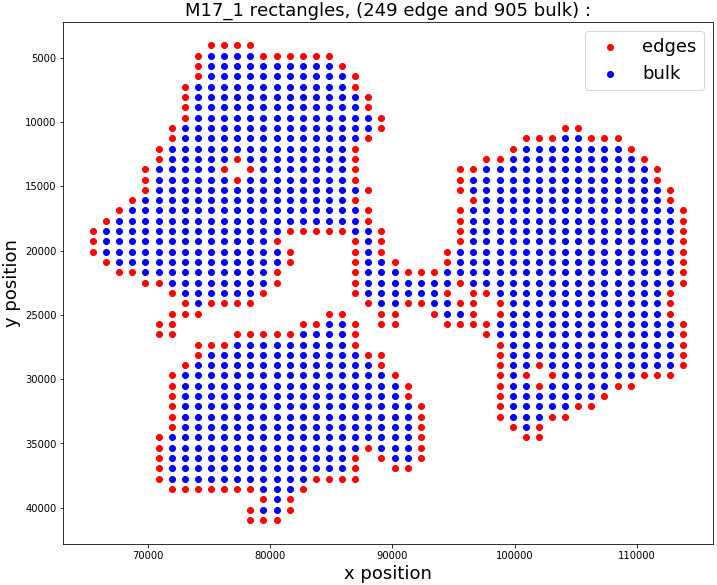
\includegraphics[width=0.95\textwidth]{images/masking/rectangle_locations_M17_1}
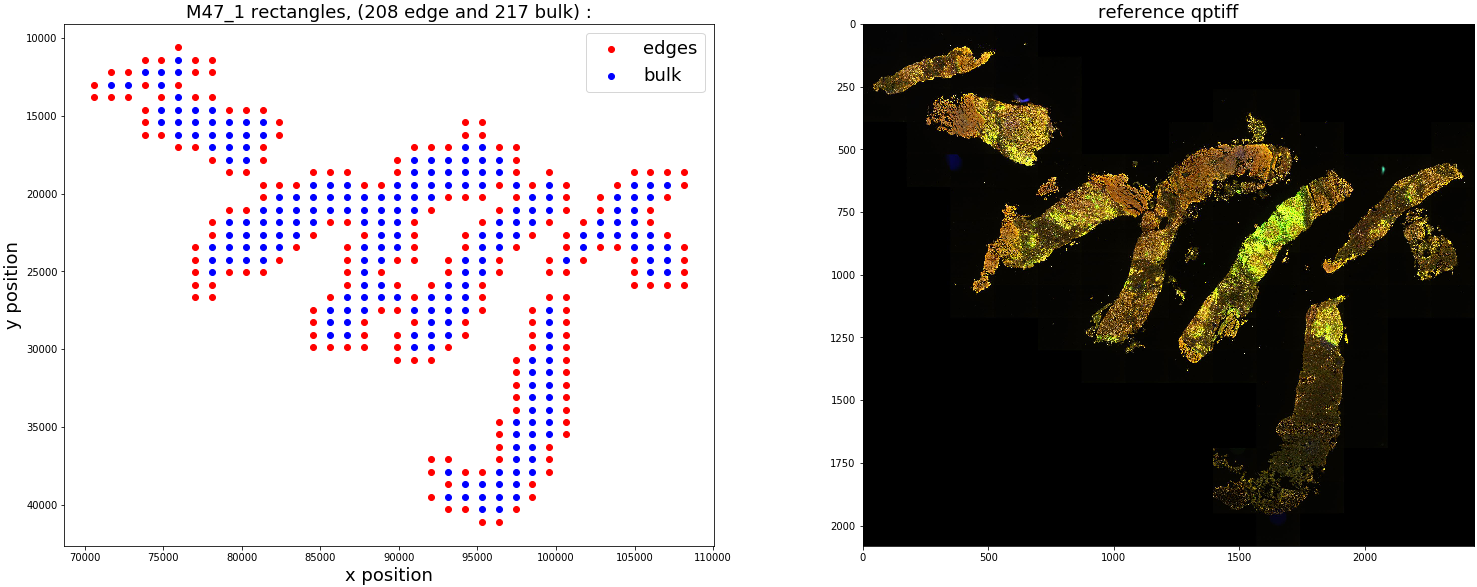
\includegraphics[width=0.95\textwidth]{images/masking/rectangle_locations_M47_1}
\caption{\footnotesize Locations of HPFs on edges of tissue (left column) next to low-resolution reference .qptiff images (right column) for samples named M3\_1 (upper row), M17\_1 (middle row), and M47\_1 (lower row). }
\label{fig:edge_HPFs}
\end{figure}

Let each raw tissue edge HPF image be represented by a three-dimensional tensor $I_{ijm}$ whose $x$, $y$, and layer coordinates are indexed by $i=1,\ldots,w$, $j=1,\ldots,l$, and $m=1,\ldots,n$, respectively (where $w$, $l$, and $n$ are the width and length of the image in pixels and the number of image layers, respectively), and whose contents are luminous fluxes in units of counts. Each image layer is first smoothed with a 5 pixel-wide Gaussian filter to remove random, small-scale variations, producing a set of smoothed image layers $S_{ijm}$. The layers of $S$ are then collapsed into histograms $H_{m}(f)$ where $f$ is the number of counts (ranging from 0 to $\fmax=65,535$ for 16-bit unsigned integers). \reffig{fig:raw_to_smoothed_to_histogram} shows $I_{ij1}$ and $S_{ij1}$ stretched from minimum to maximum in grayscale and the $H_{1}$ histogram for the first layer of a single HPF on the edge of the tissue in the sample called M21\_1. 

\begin{figure}[!ht]
\centering
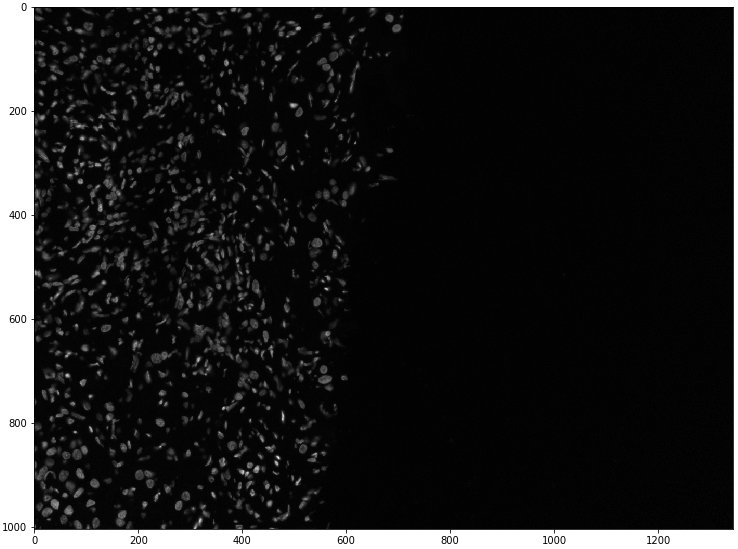
\includegraphics[width=0.45\textwidth]{images/masking/example_raw_image}
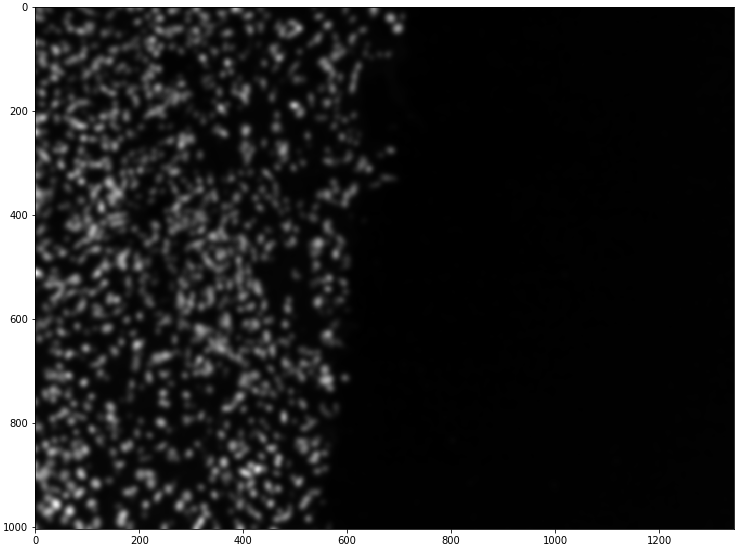
\includegraphics[width=0.45\textwidth]{images/masking/example_smoothed_image}
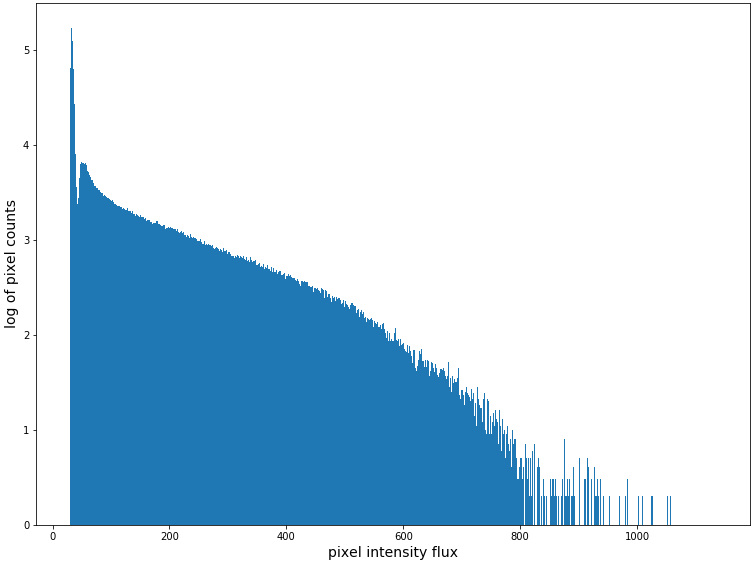
\includegraphics[width=0.45\textwidth]{images/masking/example_histogram}
\caption{\footnotesize Raw image $I_{ij1}$ (upper left), smoothed image $S_{ij1}$ (upper right), and pixel intensity histogram $H_{1}$ (lower) for the first layer of an example tissue-edge HPF in the sample named M21\_1. (Note that the histogram is shown with a logarithmic y-axis.)}
\label{fig:raw_to_smoothed_to_histogram}
\end{figure}

The background pixels appear as peaks near the low edges of the $H_{m}(f)$ histograms: finding a threshold above which pixels are likely to show tissue amounts to finding the extents of those low peaks. To this end we employ Otsu's thresholding algorithm \cite{4310076}, which determines the threshold $T$ that maximizes the inter-class variance $\sigma^2(t)$ as a function of the threshold $t$ separating the signal and background classes in each $H$ (where the layer index $m$ has been suppressed because the procedure is identical and independent for all layers),
\begin{equation}
T = \argmax{ \left\{ \sigma^2(t) \right\} } = \argmax{ \left\{ w_{b}(t) w_{s}(t) \left[ \frac{1}{w_{b}(t)}\sum_{f=0}^{t-1} f H(f) - \frac{1}{w_{s}(t)}\sum_{f=t}^{\fmax} f H(f) \right]^2 \right\} },
\label{eq:otsu_threshold_def}
\end{equation}  
where $w_{b}(t) = \sum_{f=0}^{t-1} H(f)$ and $w_{s}(t) = \sum_{f=t}^{\fmax} H(f)$ are variance weights for the background and signal classes, respectively.

We apply this algorithm iteratively to each $H(f)$ to find $K$ points of separation $T_{1}, \ldots, T_{K}$ between different categories of pixel intensities. Each successive $T_{k}$ is defined as the result of applying \refeq{eq:otsu_threshold_def} to the subset of $H$ bounded above by the previous threshold $T_{k-1}$, where $T_{0}=\fmax$ and summations to $\fmax$ in \refeq{eq:otsu_threshold_def} are replaced by summations to $T_{k-1}$ for each $k=1,\ldots,K$. Iteration continues until no more pixels are left with flux $f<T_{K+1}$, so the value of $K$ varies for each $H$.

We define a background pixel flux distribution $B(t)$ as the subset of $H$ that is bounded above by the flux $t$, and we define the population skew (or third standardized moment) of $B(t)$ as $\widetilde{\mu}(t)$. The optimal background threshold flux $\tau$ for a given $H$ is then chosen as the member of the Otsu threshold set which exhibits the maximal value of the local slope of the $\widetilde{\mu}$ function weighted by $\widetilde{\mu}(t)$, like
\begin{equation}
\tau = \argmax{\left[ \xi(k) \right]} = \argmax{ \left[ \frac{ \widetilde{\mu}(T_{k}+1) - \widetilde{\mu}(T_{k}-1) }{ 2 \widetilde{\mu}(T_{k}) } \right] } .
\label{eq:otsu_choice_def}
\end{equation}

This method tends to choose thresholds resulting in $B(\tau)$ with large local $\widetilde{\mu}$ slopes and small values of $\widetilde{\mu}(\tau)$, indicating a left-weighted peak near $\tau$ that is relatively clustered around a single mean value, as would be expected for approximately-Gaussian background noise at the low end of $H$. \reffig{fig:histograms_with_otsu_thresholds} shows the thresholds $T_{k}$ overlaid on partial pixel intensity histograms for several $H$ distributions from the example dataset named M21\_1, as well as their corresponding $\widetilde{\mu}(T_{k})$ values and weighted and unweighted local $\widetilde{\mu}$ slopes. It can be seen that the choice defined by \refeq{eq:otsu_choice_def} usually selects a $B(\tau)$ that is, visually, the lowest peak in $H$.

\begin{figure}[!ht]
\centering
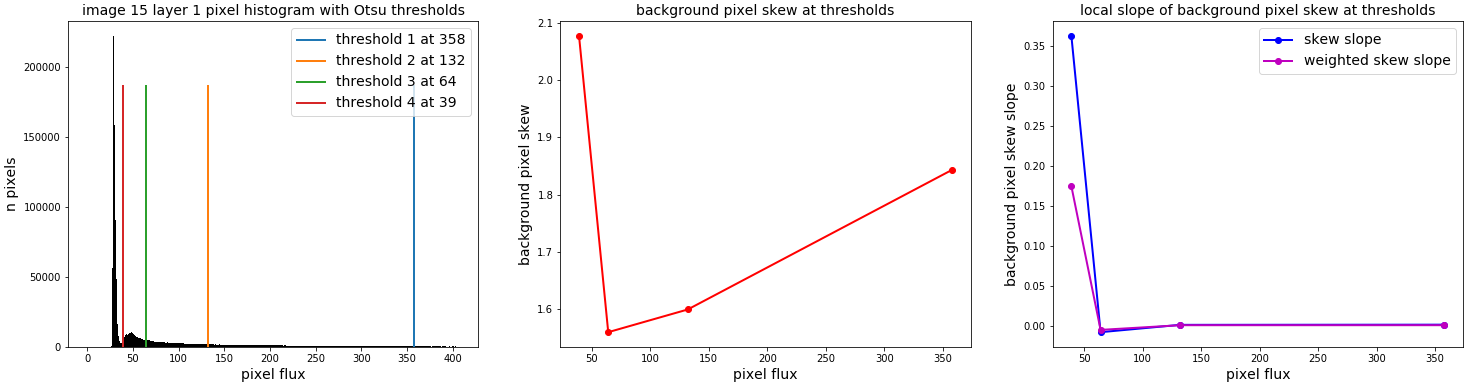
\includegraphics[width=0.9\textwidth]{images/masking/thresholds_image_15_layer_1}
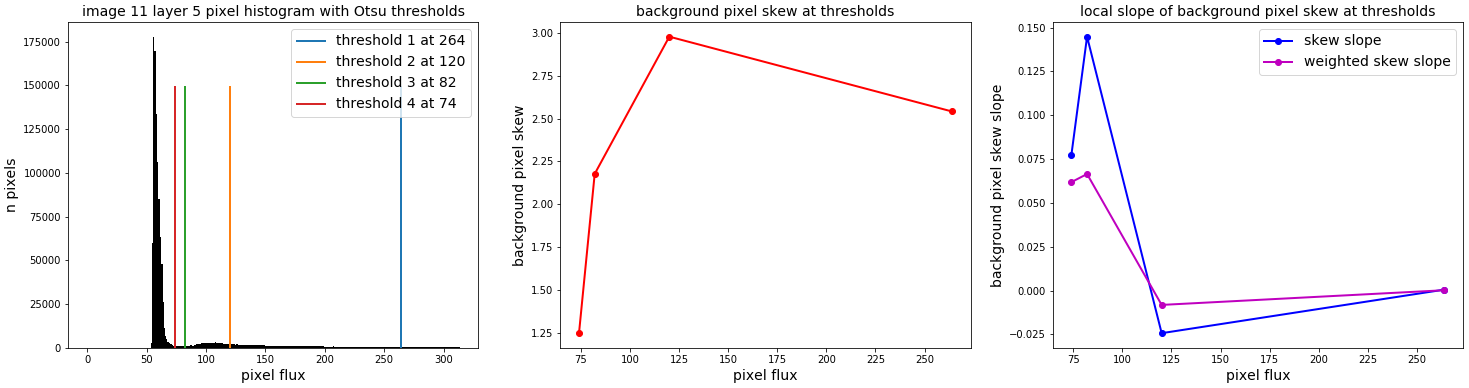
\includegraphics[width=0.9\textwidth]{images/masking/thresholds_image_11_layer_5}
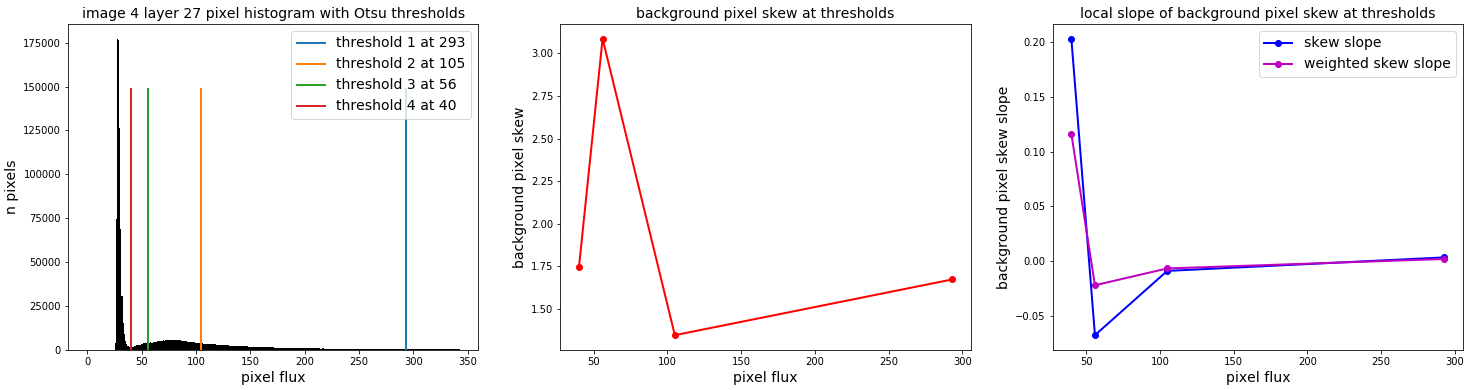
\includegraphics[width=0.9\textwidth]{images/masking/thresholds_image_4_layer_27}
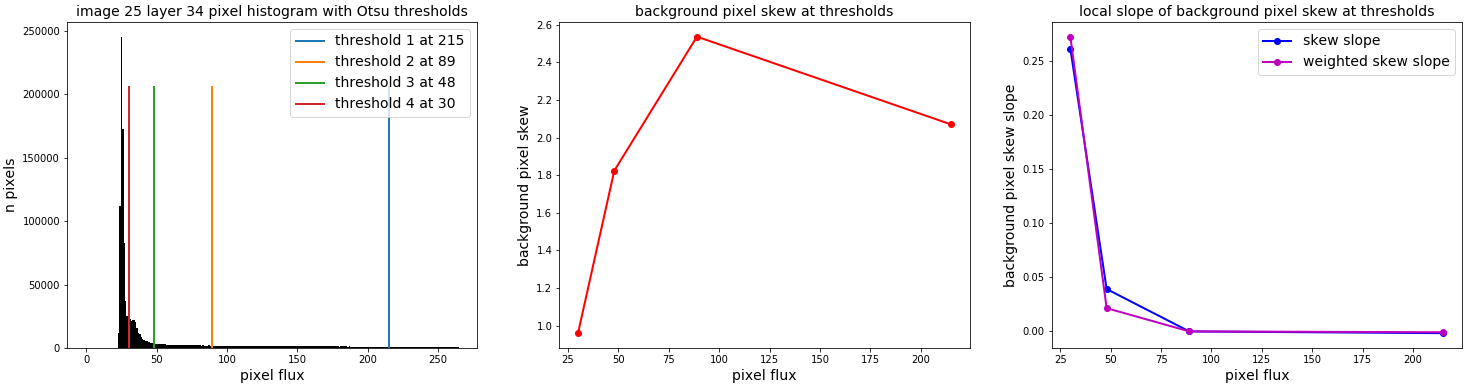
\includegraphics[width=0.9\textwidth]{images/masking/thresholds_image_25_layer_34}
\caption{\footnotesize Partial $H$ histograms with $T_{k}$ thresholds overlaid (left column), $\widetilde{\mu}(T_{k})$ values (middle column), and ``skew slope'' ($0.5*\left[\widetilde{\mu}(T_{k}+1) - \widetilde{\mu}(T_{k}-1)\right]$) and ``weighted skew slope'' ($\xi(k)$) values (right column), for the 1st, 5th, 27th, and 34th layers of the 16th, 12th, 5th, and 26th tissue edge HPFs in the sample named M21\_1 (rows upper to lower, respectively).}
\label{fig:histograms_with_otsu_thresholds}
\end{figure}

For each sample, a set of final background thresholds per layer $\Tau_{m}$ is chosen as the mean of the $\tau$ values found for each tissue edge HPF layer. Figures~\ref{fig:threshold_distributions_1} and ~\ref{fig:threshold_distributions_2} show the distributions of $\tau$ values observed in several example sample layers, next to the sum of the $B(\tau)$ histograms for all edge HPFs in the sample. The thresholding method used produces fairly regular distributions of the final background pixel flux distributions. \reffig{fig:all_sample_thresholds} shows severals statistics describing the $\Tau_{m}$ values found for all 46 of the Vectra 3.0 microscope samples analyzed; there is clear dependence on the broadband filter region, and there is nonzero but regular variation amongst the values found by layer for each sample.

\begin{figure}[!ht]
\centering
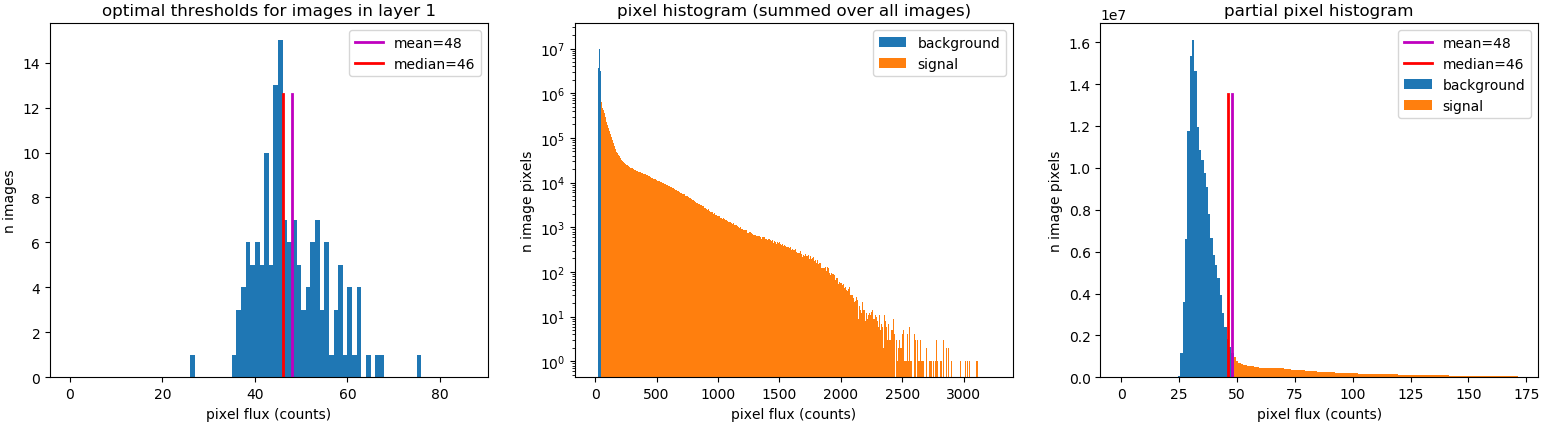
\includegraphics[width=0.80\textwidth]{images/masking/M1_1_layer_1_background_threshold_plots}
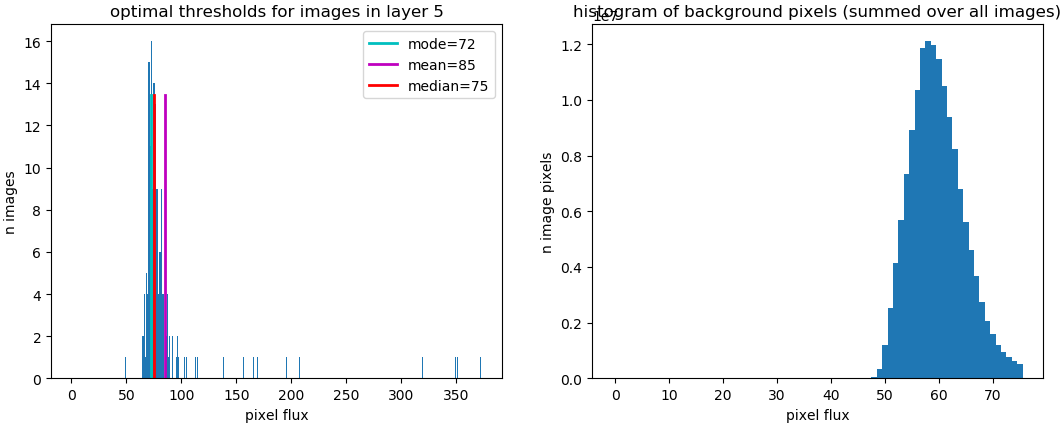
\includegraphics[width=0.80\textwidth]{images/masking/M3_1_layer_5_background_threshold_plots}
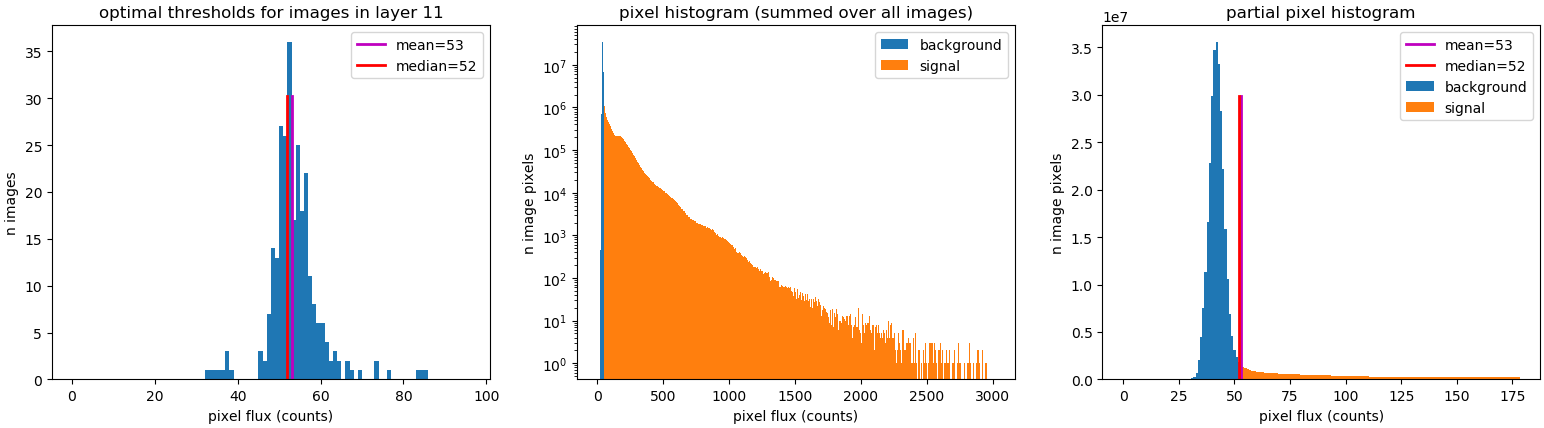
\includegraphics[width=0.80\textwidth]{images/masking/M4_2_layer_11_background_threshold_plots}
\caption{\footnotesize Distribution of $\tau$ values (left column) and summed $B(\tau)$ histograms (right column) for all tissue edge HPFs in the 1st layer of the sample named M1\_1 (upper row), 5th layer of the sample named M3\_1 (middle row), and 11th layer of the sample named M4\_2 (lower row).}
\label{fig:threshold_distributions_1}
\end{figure}

\begin{figure}[!ht]
\centering
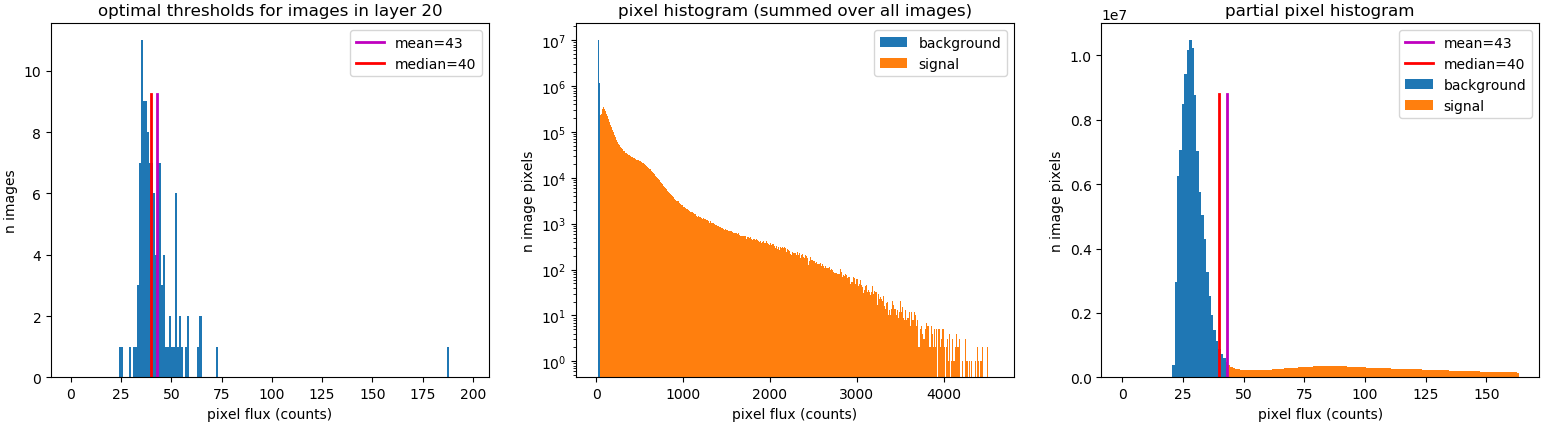
\includegraphics[width=0.80\textwidth]{images/masking/M6_1_layer_20_background_threshold_plots}
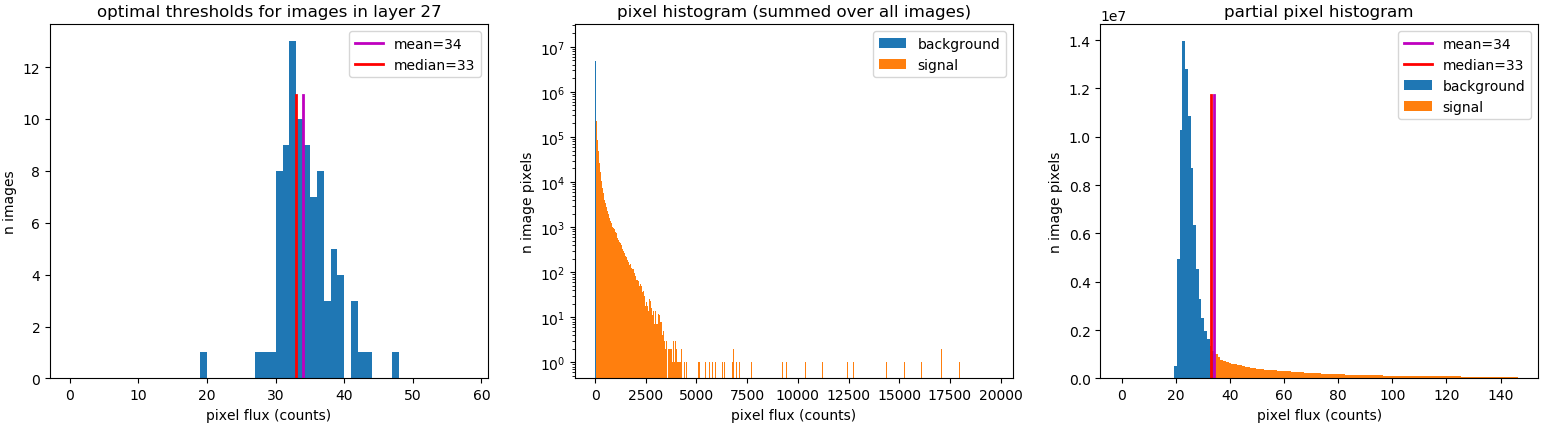
\includegraphics[width=0.80\textwidth]{images/masking/M10_2_layer_27_background_threshold_plots}
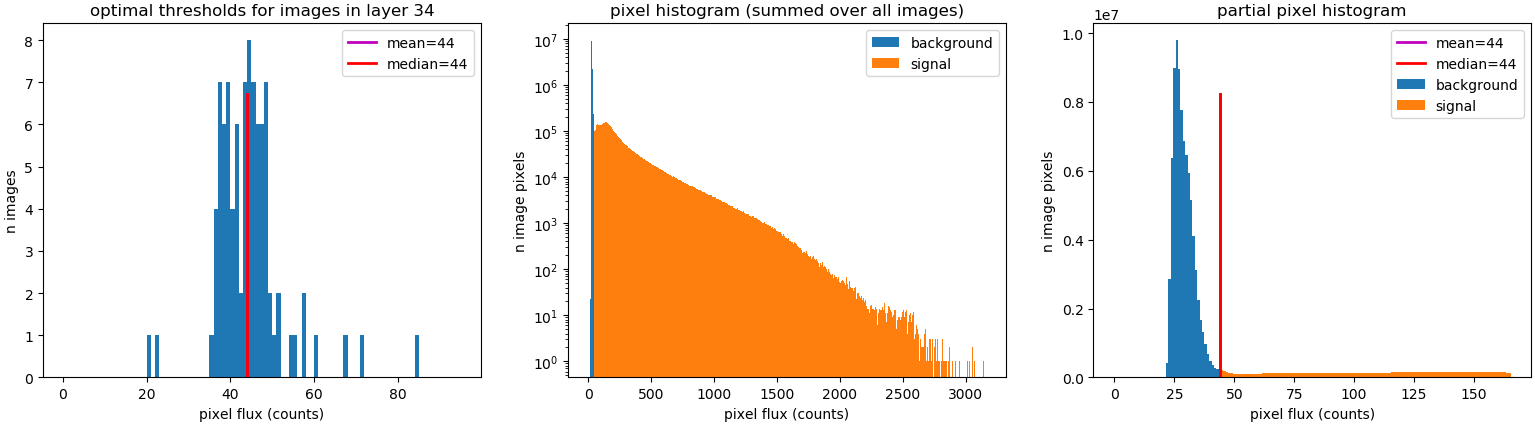
\includegraphics[width=0.80\textwidth]{images/masking/M11_1_layer_34_background_threshold_plots}
\caption{\footnotesize Distribution of $\tau$ values (left column) and summed $B(\tau)$ histograms (right column) for all tissue edge HPFs in the 20th layer of the sample named M6\_1 (upper row), 27th layer of the sample named M10\_2 (middle row), and 34th layer of the sample named M11\_1 (lower row).}
\label{fig:threshold_distributions_2}
\end{figure}

\begin{figure}[!ht]
\centering
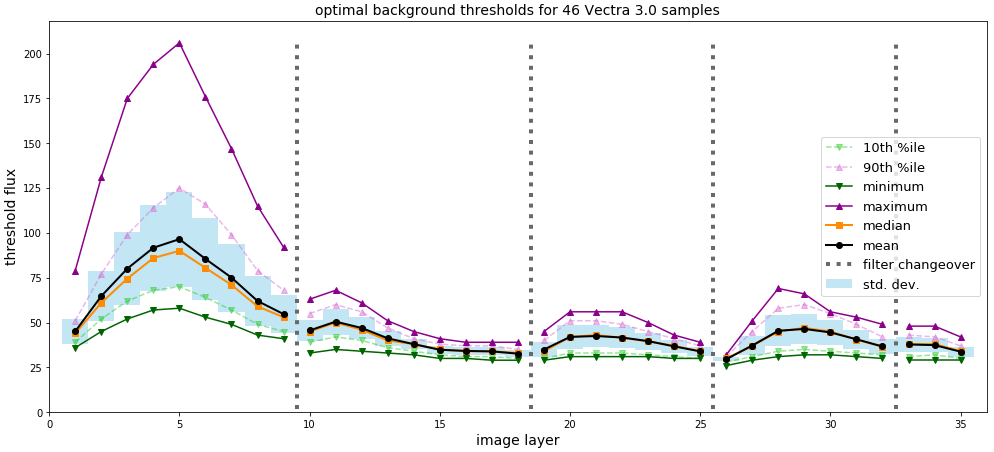
\includegraphics[width=\textwidth]{images/masking/optimal_background_thresholds_batches_3-9_samples}
\caption{\footnotesize Maximum, minimum, 10th percentile, 90th percentile, median, mean, and standard deviation of $\Tau_{m}$ values determined from tissue edge HPFs for 46 Vectra 3.0 melanoma samples.}
\label{fig:all_sample_thresholds}
\end{figure}

%%%%%%%%%%% Producing image masks subsection
\subsection{Producing image masks}
\label{ssec:producing_image_masks}

The $\Tau_{m}$ values found for each sample can be used to mask background pixels out of arbitrary images from the same sample, layer-by-layer. Given a smoothed raw image $S_{ijm}$, an initial binary mask $M^{\prime}_{ijm}$ can be defined by a simple threshold at $\Tau_{m}$ as
\begin{equation}
M^{\prime}_{ijm} = 
\begin{cases} 
      0 & S_{ijm} \leq \Tau_{m} \\
      1 & S_{ijm} > \Tau_{m} 
\end{cases}
 .
\end{equation}
Multiplying an image by this binary mask will effectively remove regions that are not bright enough to be identified as fluorescent tissue.

The smoothed image (as opposed to the raw image) is used to reduce the granularity of the initial mask, but the binary thresholding alone is not sufficient to produce a mask that uniformly describes bulk tissue regions of images. The initial $M^{\prime}_{ijm}$ masks are therefore transformed using image morphological operations \cite{opencv_mt} to produce larger and less isolated regions of identified signal and background. The operations used are of the ``open'' and ``close'' types, which are themselves compositions of ``erosion'' and ``dilation'' operations: an ``open'' operation is an erosion followed by a dilation, both with the same structure element, and a ``close'' operation is a dilation followed by an erosion with the same structure element.

The initial mask image is first closed and then opened with an elliptical structure element of extent $9 \times 9$ pixels to fill in small holes that are surrounded by larger areas and remove any small, isolated areas. Another close and open is then performed with an elliptical element of size $16 \times 16$ pixels to serve the same purpose on a medium scale. The overall bulk of the mask is then defined by a single close operation with an elliptical element of size $25 \times 25$ pixels. The edges of this bulk are refined, and small areas outside of it are removed, by opening three times with the $9 \times 9$ pixel structure element, to produce the final binary mask $M_{ijm}$. This sequence of operations is pictured in \reffig{fig:morphological_transformations} for an example image layer. 

\begin{figure}[!ht]
\centering
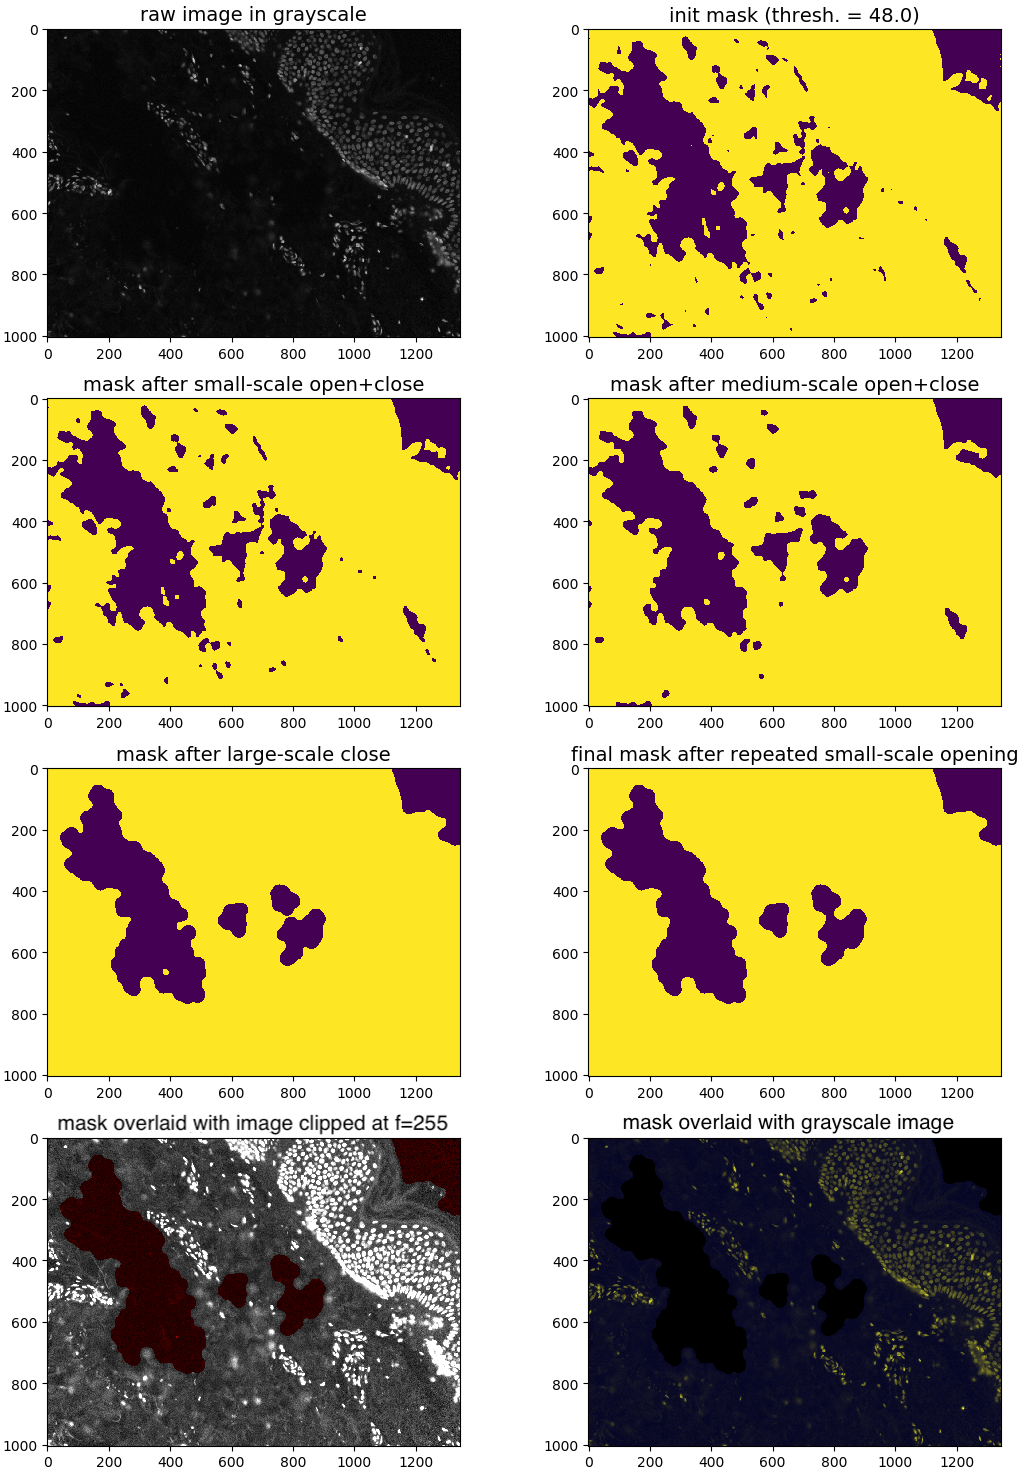
\includegraphics[width=0.80\textwidth]{images/masking/image_286_layer_9_masks}
\caption{\footnotesize Example application of morphological transformations used to refine initial binary masks. Image shown is from layer 9 of the sample named M14\_1. The raw image stretched from maximum to minimum in grayscale is shown in the upper left, and the initial mask layer $M^{\prime}_{ij9}$ from thresholding at $\Tau_{9}=48$ is shown in the upper right. The results of applying the small-scale (left) and medium-scale (right) close and open operations are shown in the second row. The result of a single large-scale close is shown in the left column of the third row. The final mask $M_{ij9}$ after the repeated small-scale open is shown in the right column of the third row. The lower row shows the final transformed mask overlaid with (left) the raw image with flux clipped at $f=255$ to show the background more brightly in red, and (right) the raw image in grayscale.}
\label{fig:morphological_transformations}
\end{figure}

To further illustrate the masking procedure and the wide variation in the initial thresholds required, three more examples of how initial masks are transformed are shown in Figures~\ref{fig:mask_example_min}, \ref{fig:mask_example_med}, and~\ref{fig:mask_example_max} for image layers whose initial thresholds represent the global minimum, median, and maximum, respectively, of the values shown in \reffig{fig:all_sample_thresholds}. Transforming the initial masks in this way tends to result in masks containing a minimal number of maximally-connected regions that correllate well with the tissue in each image, including smaller-scale features of the bulk but removing them from more isolated areas. The transformations described are performed for all image layers simultaneously on a GPU to maximize efficiency. 

\begin{figure}[!ht]
\centering
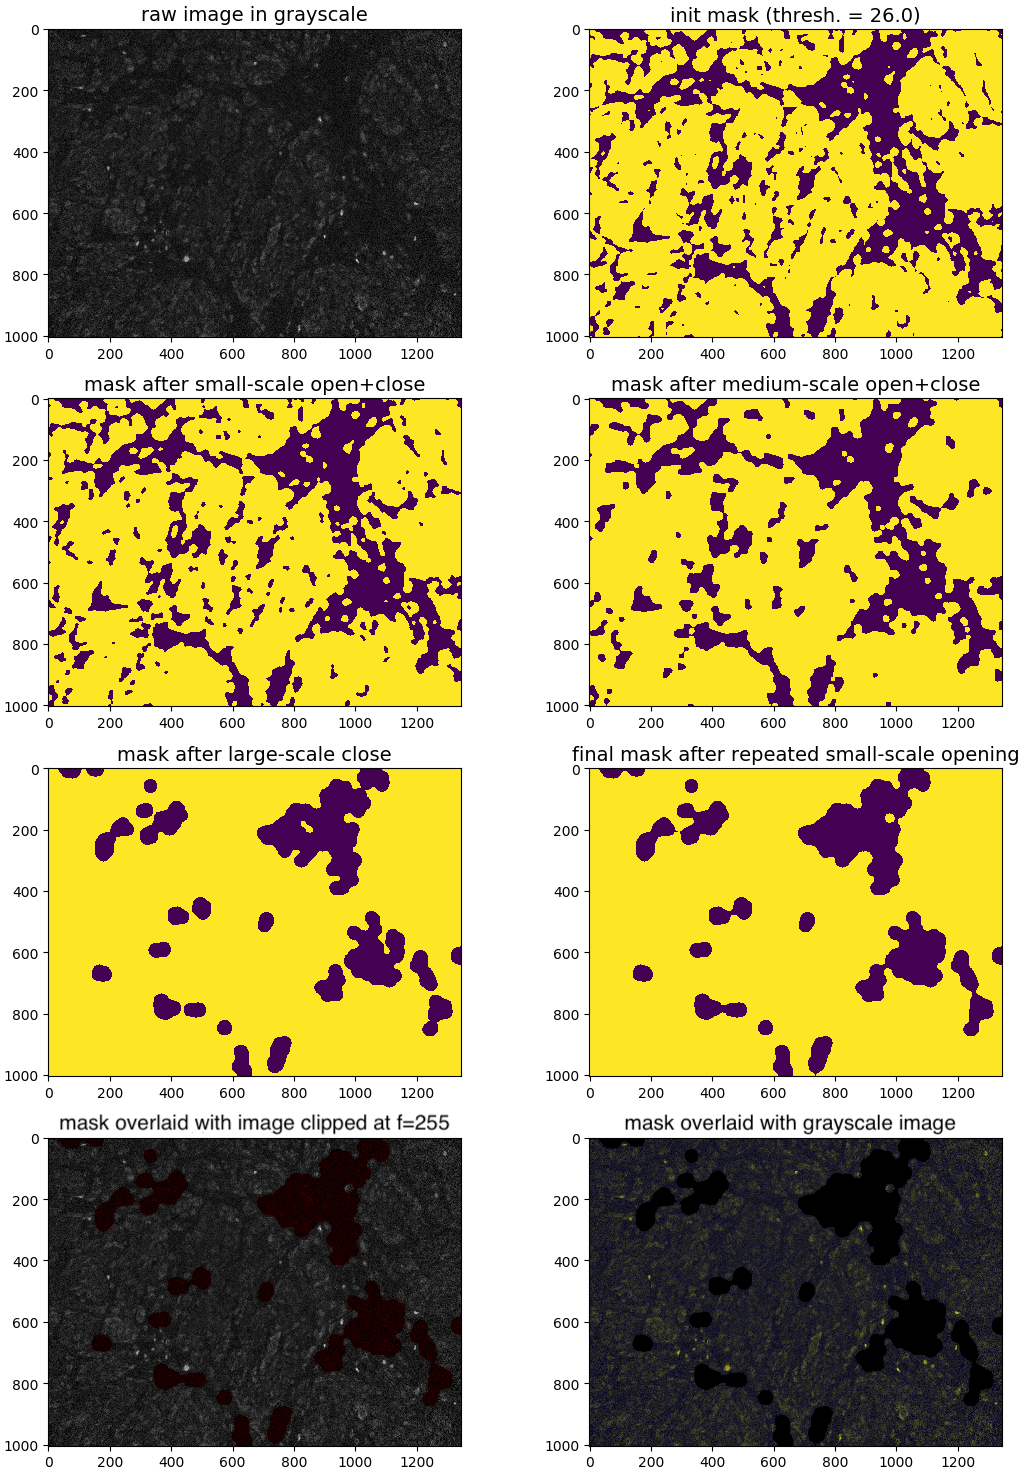
\includegraphics[width=0.80\textwidth]{images/masking/image_110_layer_26_masks}
\caption{\footnotesize Example application of morphological transformations used to refine initial binary masks. Image shown is from layer 26 of the sample named M11\_1. The raw image stretched from maximum to minimum in grayscale is shown in the upper left, and the initial mask layer $M^{\prime}_{ij26}$ from thresholding at $\Tau_{26}=26$ is shown in the upper right. The results of applying the small-scale (left) and medium-scale (right) close and open operations are shown in the second row. The result of a single large-scale close is shown in the left column of the third row. The final mask $M_{ij26}$ after the repeated small-scale open is shown in the right column of the third row. The lower row shows the final transformed mask overlaid with (left) the raw image with flux clipped at $f=255$ to show the background more brightly in red, and (right) the raw image in grayscale.}
\label{fig:mask_example_min}
\end{figure}

\begin{figure}[!ht]
\centering
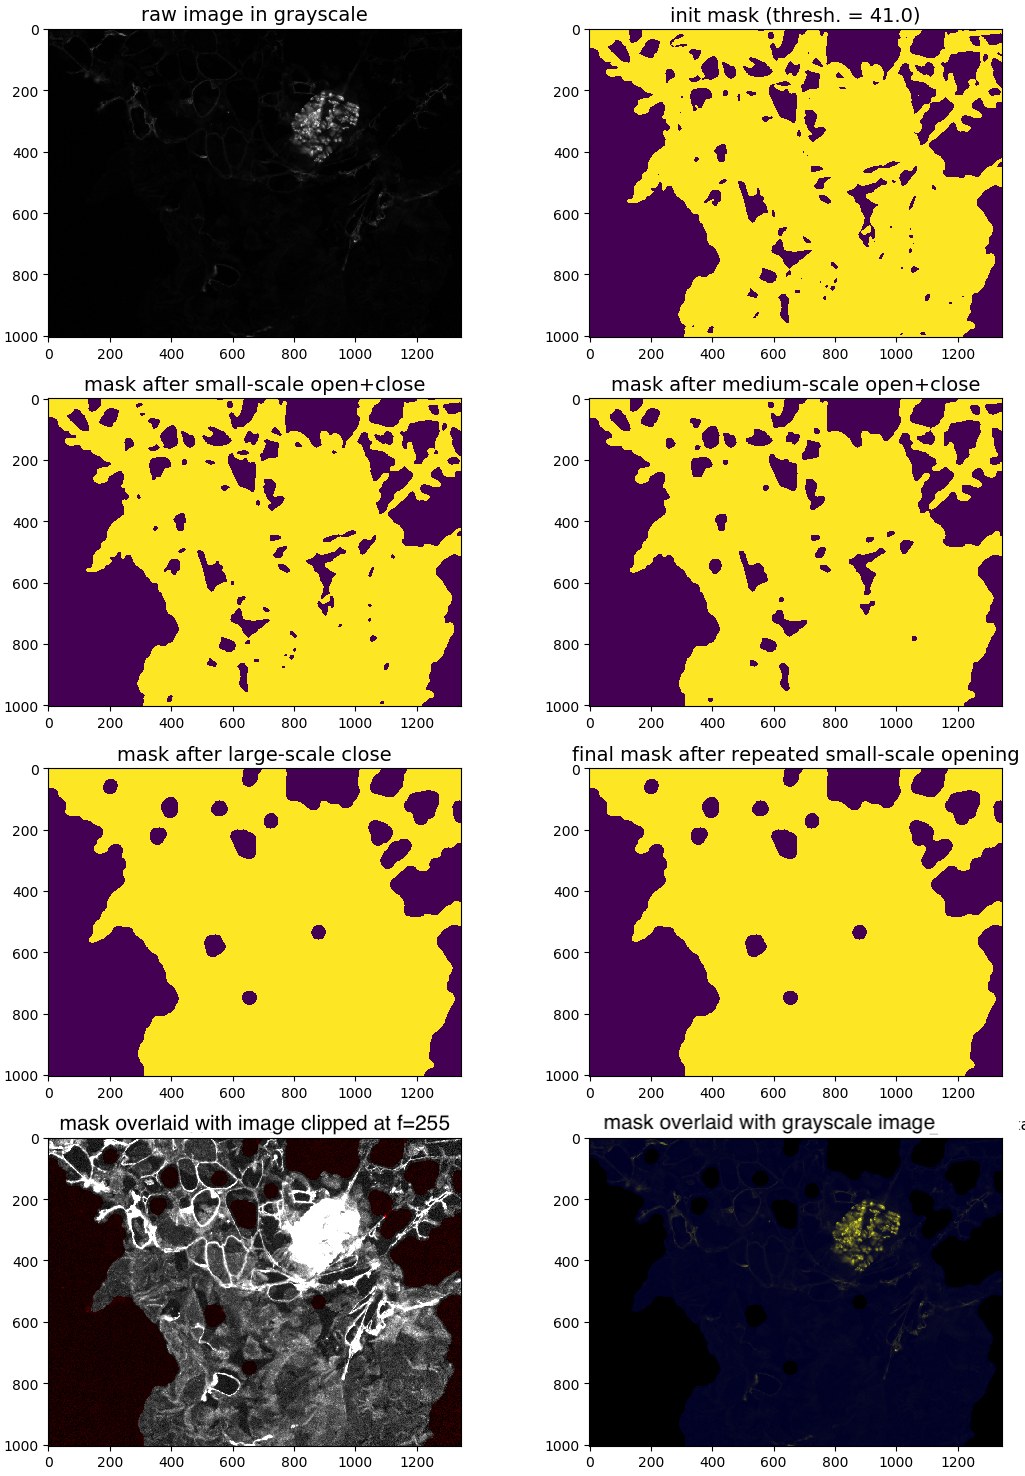
\includegraphics[width=0.80\textwidth]{images/masking/image_6455_layer_29_masks}
\caption{\footnotesize Example application of morphological transformations used to refine initial binary masks. Image shown is from layer 29 of the sample named M43\_1. The raw image stretched from maximum to minimum in grayscale is shown in the upper left, and the initial mask layer $M^{\prime}_{ij29}$ from thresholding at $\Tau_{29}=41$ is shown in the upper right. The results of applying the small-scale (left) and medium-scale (right) close and open operations are shown in the second row. The result of a single large-scale close is shown in the left column of the third row. The final mask $M_{ij29}$ after the repeated small-scale open is shown in the right column of the third row. The lower row shows the final transformed mask overlaid with (left) the raw image with flux clipped at $f=255$ to show the background more brightly in red, and (right) the raw image in grayscale.}
\label{fig:mask_example_med}
\end{figure}

\begin{figure}[!ht]
\centering
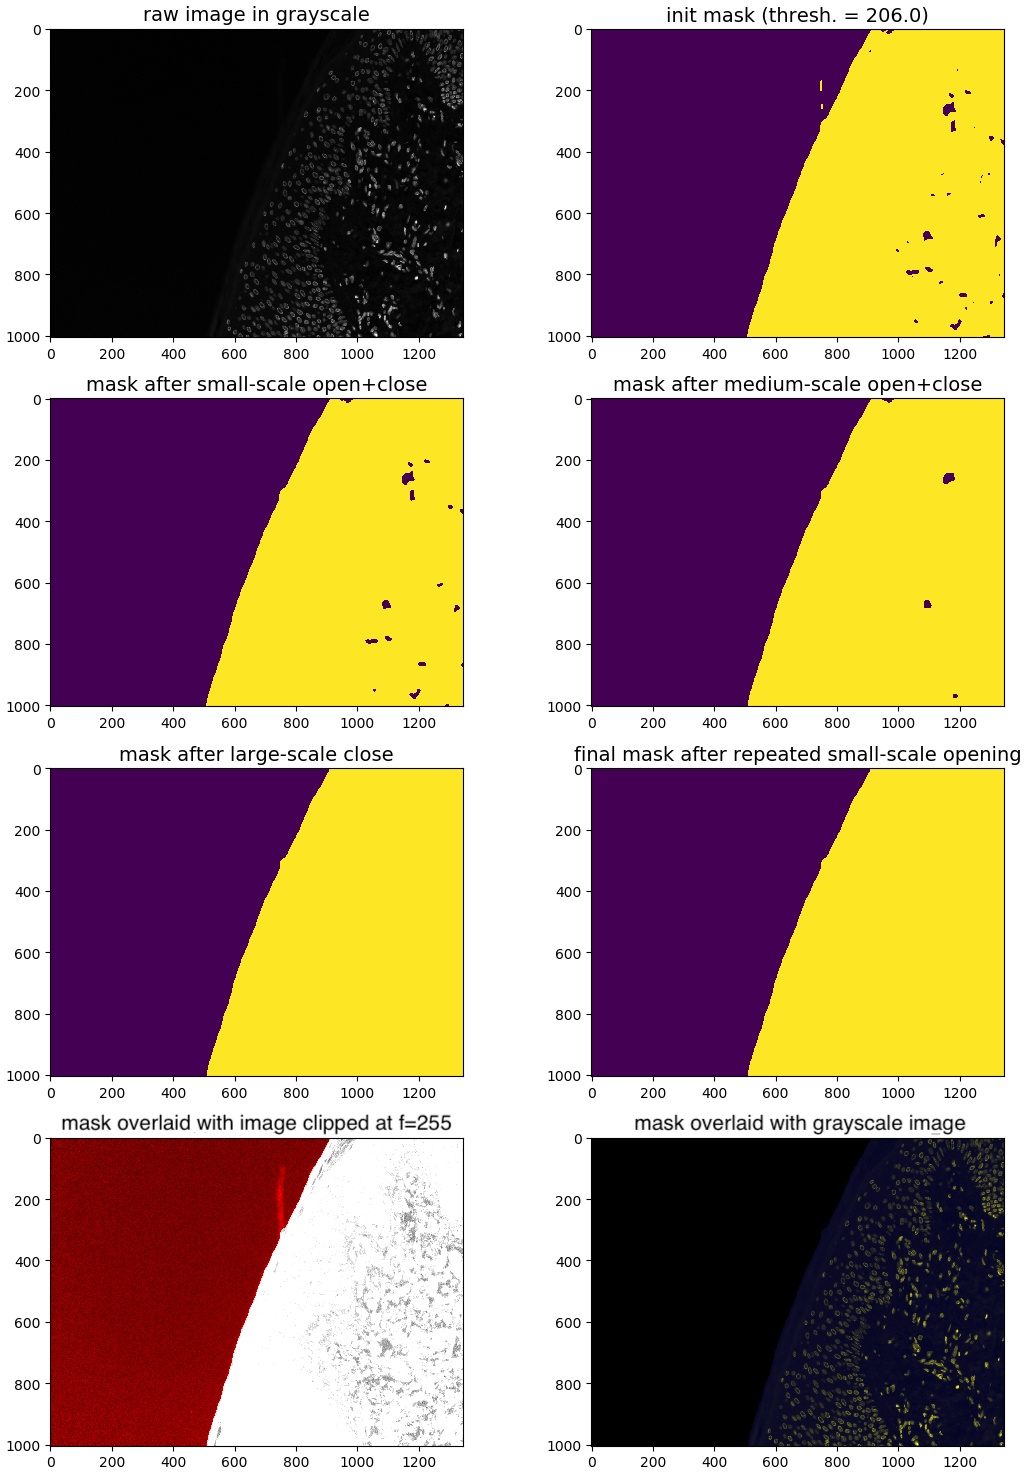
\includegraphics[width=0.80\textwidth]{images/masking/image_9941_layer_5_masks}
\caption{\footnotesize Example application of morphological transformations used to refine initial binary masks. Image shown is from layer 5 of the sample named M9\_1. The raw image stretched from maximum to minimum in grayscale is shown in the upper left, and the initial mask layer $M^{\prime}_{ij5}$ from thresholding at $\Tau_{5}=206$ is shown in the upper right. The results of applying the small-scale (left) and medium-scale (right) close and open operations are shown in the second row. The result of a single large-scale close is shown in the left column of the third row. The final mask $M_{ij5}$ after the repeated small-scale open is shown in the right column of the third row. The lower row shows the final transformed mask overlaid with (left) the raw image with flux clipped at $f=255$ to show the background more brightly in red, and (right) the raw image in grayscale.}
\label{fig:mask_example_max}
\end{figure}

\clearpage

%%%%%%%%%%%%%%%%%%%%%%%%%%%%%%%%%% MEASURING FLATFIELD CORRECTIONS SECTION %%%%%%%%%%%%%%%%%%%%%%%%%%%%%%%%%%
\section{Measuring Flatfield Corrections}
\label{sec:measuring_flatfield_corrections}

The illumination variation is measured using only a subset of all the HPF images in a sample to make the highest quality estimation of the effects in the fluorescent tissue alone. First, any images located on the edges of tissue (like those pictured in red in the left column of \reffig{fig:edge_HPFs}) are excluded. Also excluded are any image layers whose masks select less than 80\% of the total pixels (that is, $\sum_{i=1}^{w}\sum_{j=1}^{l}M_{ijm}<0.8*(w*l)$) so that only images primarily showing tissue are stacked. 

This cut on the fraction of selected pixels reduces the phenomenon of overselecting noise in systematically brightly-illuminated regions of otherwise largely empty HPFs. The fraction of 80\% was chosen because it introduces only minimal bias to the variation in the number or location of the images that are stacked in each layer, as shown in Figures~\ref{fig:selected_pixel_fraction_cut_1} and~\ref{fig:selected_pixel_fraction_cut_2}. With no requirement on the selected pixel fraction, a systematic bias to the lower right hand corner of the images is observed. This bias persists with the cut at 20\%, and a different systematic bias toward the image centers is observed with the cut at 50\%. The cut at 80\% is the smallest value of the cut that shows less bias to any region, and which also does not increase the spread in how many images are stacked in every image layer.

\begin{figure}[!ht]
\centering
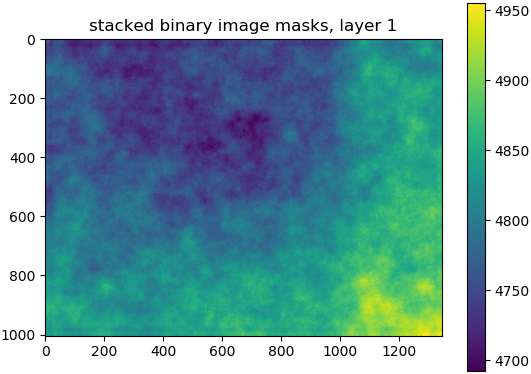
\includegraphics[width=0.45\textwidth]{images/measuring_flatfield_corrections/example_mask_stack_layer_1_cut_at_0_00}
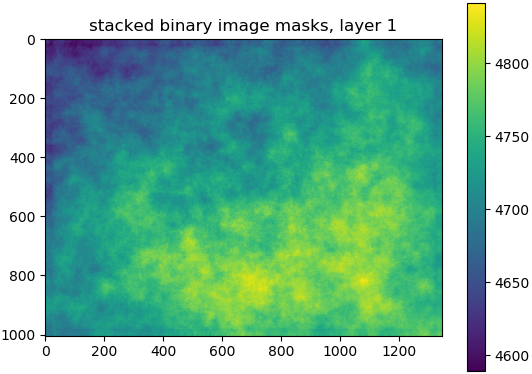
\includegraphics[width=0.45\textwidth]{images/measuring_flatfield_corrections/example_mask_stack_layer_1_cut_at_0_20}
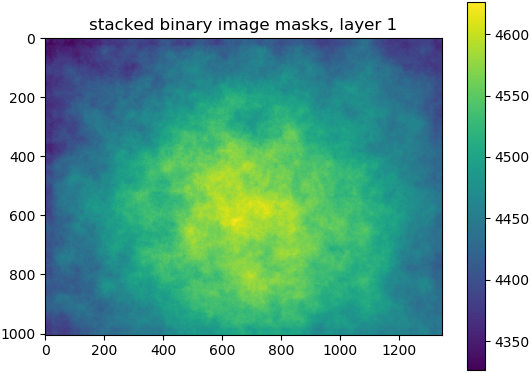
\includegraphics[width=0.45\textwidth]{images/measuring_flatfield_corrections/example_mask_stack_layer_1_cut_at_0_50}
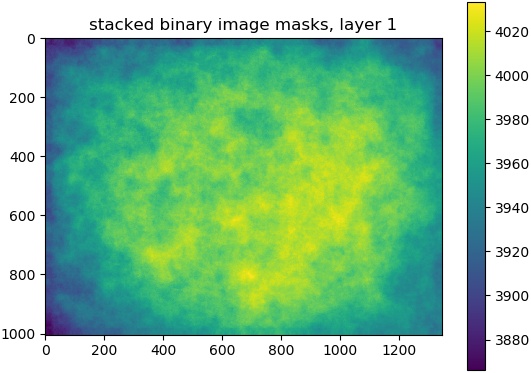
\includegraphics[width=0.45\textwidth]{images/measuring_flatfield_corrections/example_mask_stack_layer_1_cut_at_0_80}
\caption{\footnotesize Numbers of masks selected to be stacked at each location in the first image layer, with the required fraction of selected pixels at 0\% (no cut, upper left), 20\% (upper right), 50\% (lower left), and 80\% (lower right). Figures shown were all produced using a set of 6,309 total initial HPFs from 11 Vectra 3.0 samples named M6\_1, M3\_1, M17\_1, M29\_1, M16\_1, M35\_1, M25\_1, M36\_1, M52\_1, M21\_1, and M14\_1.}
\label{fig:selected_pixel_fraction_cut_1}
\end{figure}

\begin{figure}[!ht]
\centering
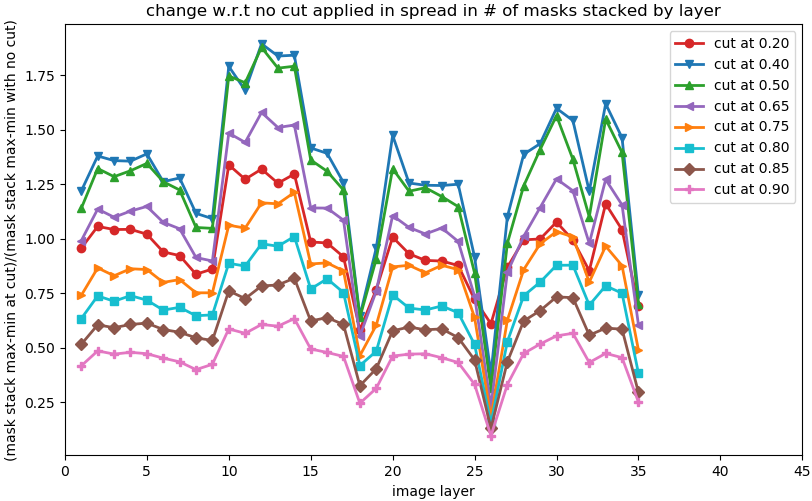
\includegraphics[width=0.80\textwidth]{images/measuring_flatfield_corrections/example_mask_stack_spreads_by_layer}
\caption{\footnotesize Difference between the maximum and minimum numbers of images selected to be stacked at any location within each image layer at different values of the selected pixel fraction requirement, divided by the spread observed with no cut applied. The line representing the cut at 80\% is the first that does not increase the spread from what is initially observed. Figure produced using a set of 6,309 total initial HPFs from 11 Vectra 3.0 samples named M6\_1, M3\_1, M17\_1, M29\_1, M16\_1, M35\_1, M25\_1, M36\_1, M52\_1, M21\_1, and M14\_1.}
\label{fig:selected_pixel_fraction_cut_2}
\end{figure} 

These requirements on the images and their masked layers define a total number of HPFs from all samples to be stacked in each layer, $N_{m}$. \reffig{fig:n_images_stacked_by_layer} shows this $N_{m}$ for the total set of Vectra 3.0 samples used to make the flatfield correction image, which consists of 22,692 initial HPFs, reduced to 19,024 HPFs after removing those on the edges of the tissue. The average $N_{m}$ across all layers was 11,508.

\begin{figure}[!ht]
\centering
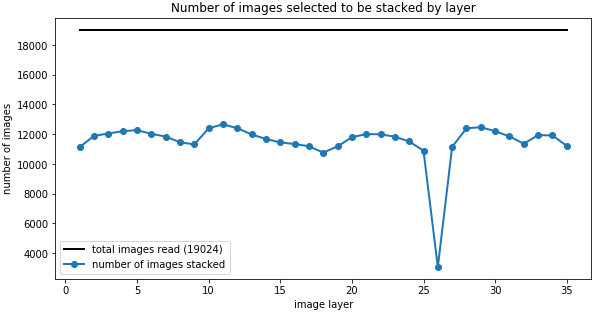
\includegraphics[width=0.80\textwidth]{images/measuring_flatfield_corrections/n_images_stacked_per_layer}
\caption{\footnotesize Number of images $N_{m}$ selected to be stacked in each layer for the set of 22,692 initial HPFs from 46 Vectra 3.0 samples.}
\label{fig:n_images_stacked_by_layer}
\end{figure} 

The previously-defined image and mask tensors $I$ and $M$ can be collected over the whole image set using a new index $\eta=1,\ldots,N_{m}$. The sum of all the masks, $\Mu_{ijm} = \sum_{\eta=1}^{N_{m}} M^{\eta}_{ijm}$ is shown in \reffig{fig:mask_stack_layers} for the first, middle, and last layers in each broadband filter region. A small bias toward selecting the lower right hand corners of the images remains in most cases. 

\begin{figure}[!ht]
\centering
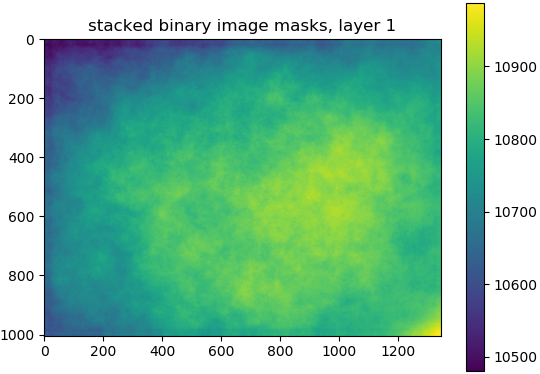
\includegraphics[width=0.3\textwidth]{images/measuring_flatfield_corrections/mask_stack_layers/mask_stack_layer_1}
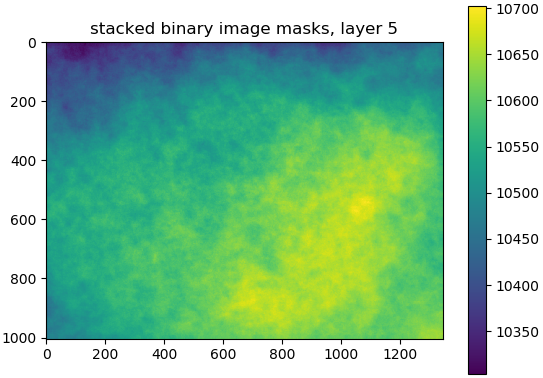
\includegraphics[width=0.3\textwidth]{images/measuring_flatfield_corrections/mask_stack_layers/mask_stack_layer_5}
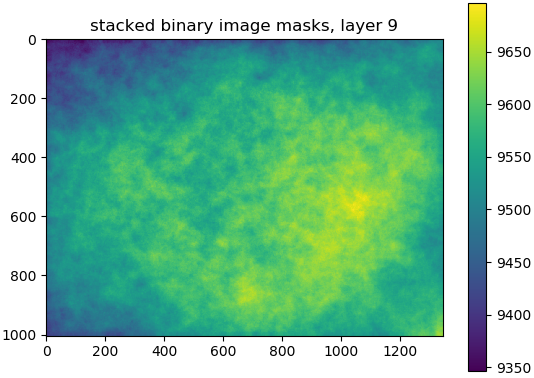
\includegraphics[width=0.3\textwidth]{images/measuring_flatfield_corrections/mask_stack_layers/mask_stack_layer_9}
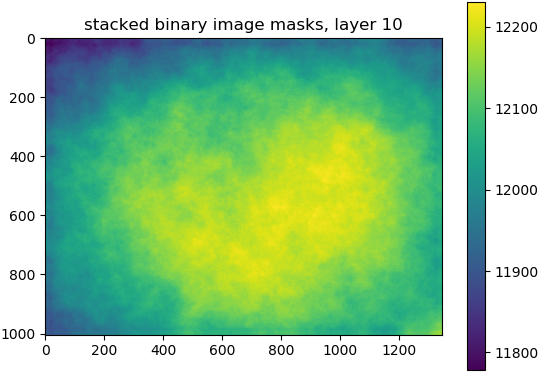
\includegraphics[width=0.3\textwidth]{images/measuring_flatfield_corrections/mask_stack_layers/mask_stack_layer_10}
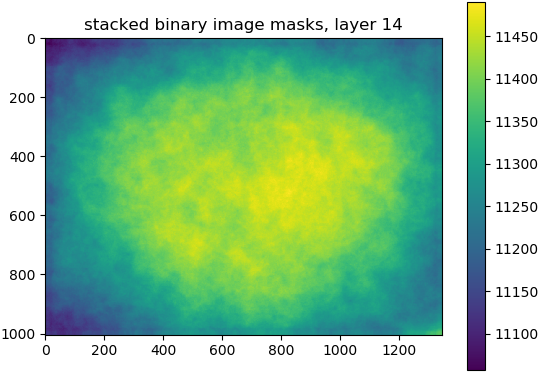
\includegraphics[width=0.3\textwidth]{images/measuring_flatfield_corrections/mask_stack_layers/mask_stack_layer_14}
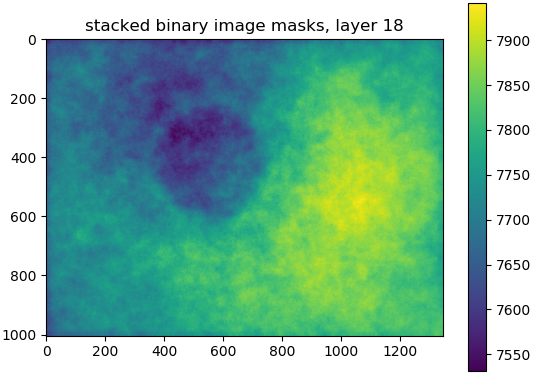
\includegraphics[width=0.3\textwidth]{images/measuring_flatfield_corrections/mask_stack_layers/mask_stack_layer_18}
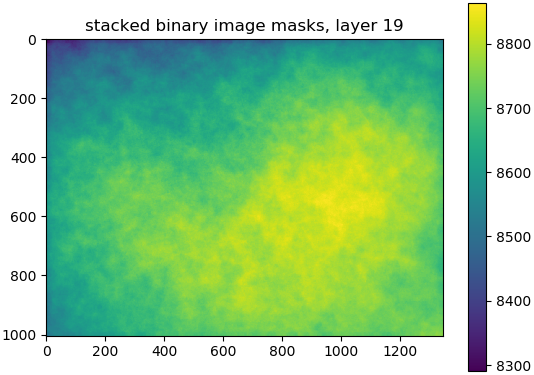
\includegraphics[width=0.3\textwidth]{images/measuring_flatfield_corrections/mask_stack_layers/mask_stack_layer_19}
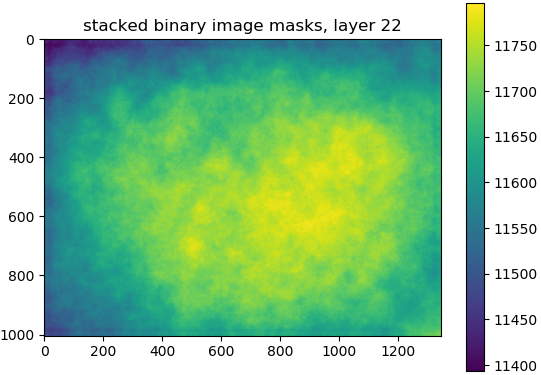
\includegraphics[width=0.3\textwidth]{images/measuring_flatfield_corrections/mask_stack_layers/mask_stack_layer_22}
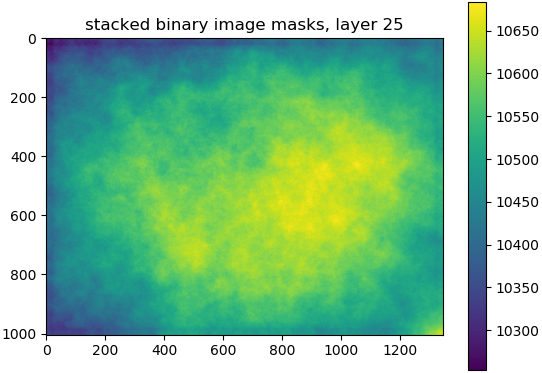
\includegraphics[width=0.3\textwidth]{images/measuring_flatfield_corrections/mask_stack_layers/mask_stack_layer_25}
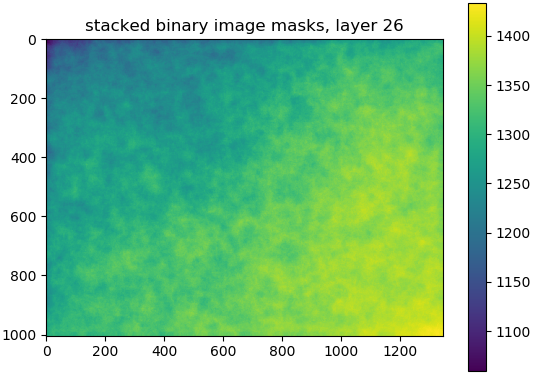
\includegraphics[width=0.3\textwidth]{images/measuring_flatfield_corrections/mask_stack_layers/mask_stack_layer_26}
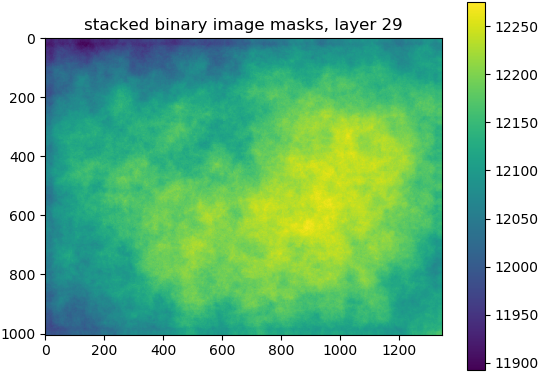
\includegraphics[width=0.3\textwidth]{images/measuring_flatfield_corrections/mask_stack_layers/mask_stack_layer_29}
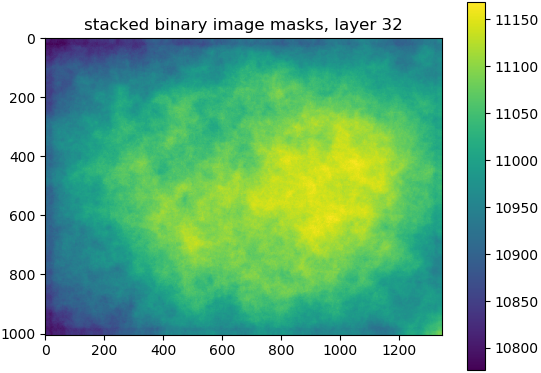
\includegraphics[width=0.3\textwidth]{images/measuring_flatfield_corrections/mask_stack_layers/mask_stack_layer_32}
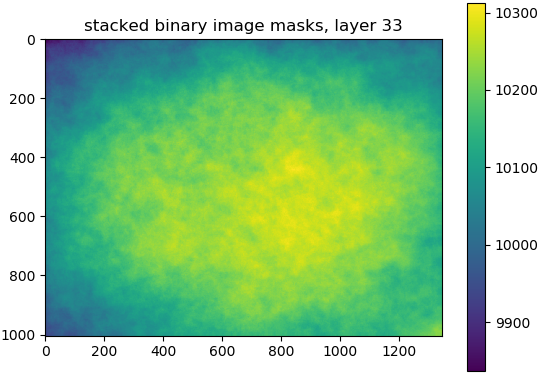
\includegraphics[width=0.3\textwidth]{images/measuring_flatfield_corrections/mask_stack_layers/mask_stack_layer_33}
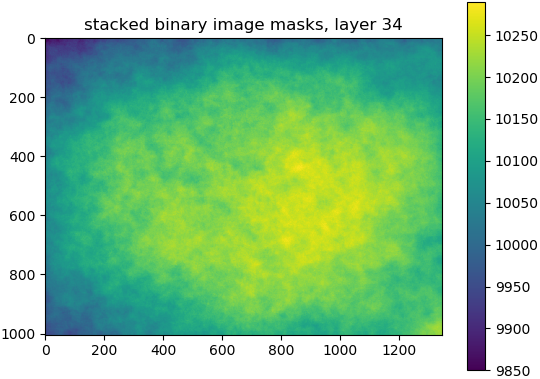
\includegraphics[width=0.3\textwidth]{images/measuring_flatfield_corrections/mask_stack_layers/mask_stack_layer_34}
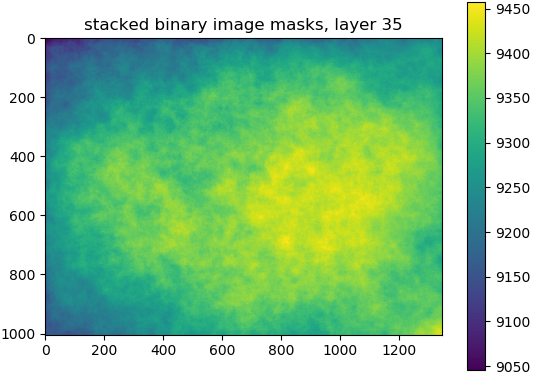
\includegraphics[width=0.3\textwidth]{images/measuring_flatfield_corrections/mask_stack_layers/mask_stack_layer_35}
\caption{\footnotesize Layers of the total stack of binary image masks, $\Mu_{ijm}$, for $m=$1, 5, 9, 10, 14, 18, 29, 22, 25, 26, 29, 32, 33, 34, and 35 from upper left to lower right, respectively. Note the differences in scales for each image.}
\label{fig:mask_stack_layers}
\end{figure}

Only the central 64\% of each fully-corrected HPF is used when pathology analyses are eventually performed, because the outer 20\% of each image's sides are used to determine the alignment and stitching of the individual HPFs to represent an entire sample \cite{Heshy}. Clipping 10\% from all sides of the image layers slightly reduces the edge effects apparent in $\Mu_{ijm}$. \reffig{fig:removing_image_edges_effect_on_mask_stacks} shows how the maximum, minimum, 5th and 95th percentile, and standard deviation of the number of masks stacked in each layer relative to the layer mean changes when the outer 36\% of the image layers are removed. The spread from the 5th to 95th percentile of the number of images stacked divided by the layer mean decreases from 2.3\% to 1.6\% on average over all layers, and the standard deviation of the number of images stacked divided by the layer mean decreases from 0.72\% to 0.49\% on average over all layers, showing that the masking and image layer selection procedures ultimately result in only very small differences in how many images contribute to measurements of the illumination variation at any point, and that those variations are even smaller in the region of interest.

\begin{figure}[!ht]
\centering
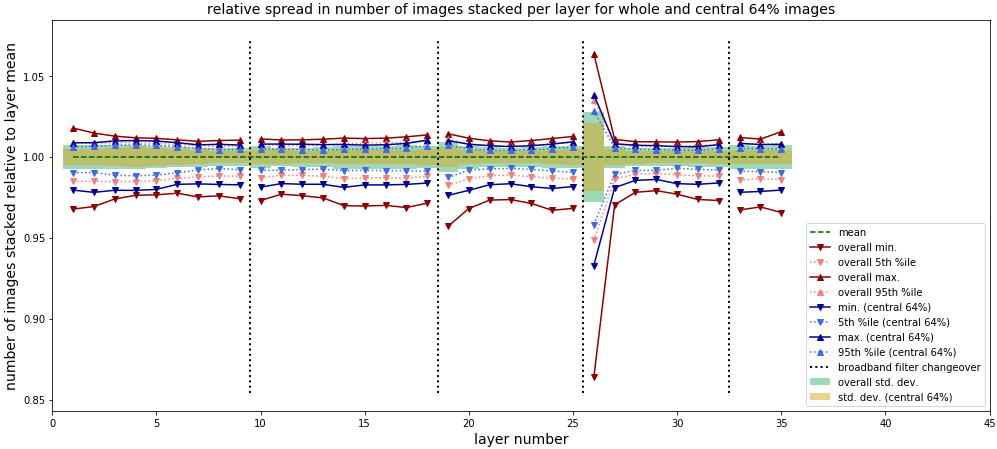
\includegraphics[width=0.90\textwidth]{images/measuring_flatfield_corrections/mask_stack_variation_reduction}
\caption{\footnotesize Maximum, minimum, 5th and 95th percentile, and standard deviation of the number of images stacked relative to the mean in each layer computed using the full images (red lines and green shading) and only the central 64\% of interest (blue lines and orange shading). The relative variation in the number of images stacked is smaller in the central region of interest.}
\label{fig:removing_image_edges_effect_on_mask_stacks}
\end{figure} 

To measure the flatfield correction factors, an initial mean image $\Iota_{ijm}$ is first defined by summing over all masked raw images and dividing by the number of images stacked, like
\begin{equation}
\Iota_{ijm} = \frac{1}{\Mu_{ijm}} \left[ \sum_{\eta=1}^{N_{m}} I^{\eta}_{ijm}*M^{\eta}_{ijm} \right] .
\end{equation}
Each layer of $\Iota$ is then smoothed using a 100 pixel-wide Gaussian filter to produce a smoothed mean image $G_{ijm}$ that describes only the large-scale variations. The final flatfield image $F_{ijm}$, whose contents are the pixel-by-pixel correction factors, is this $G$ image, with each layer normalized by its mean,
\begin{equation}
F_{ijm} = G_{ijm} \left( \frac{w*l}{\sum_{i=0}^{w-1}\sum_{j=0}^{l-1}G_{ijm}} \right) ,
\end{equation}
so that applying the corrections only changes the relative illumination within each layer. 

%%%%%%%%%%%%%%%%%%%%%%%%%%%%%%%%%%%%%%%%%%%%%% RESULTS SECTION %%%%%%%%%%%%%%%%%%%%%%%%%%%%%%%%%%%%%%%%%%%%%%
\section{Results}
\label{sec:results}

The flatfield image $F$ describes the systematic variations in the amount of illumination observed in the regions of HPF images showing fluorescent tissue. Applying the correction factors the $F$ image contains is shown to decrease the amount of illumination variation observed over a large and independent sample of identically masked and selected HPFs. The addition of image layer masking and selection is shown to improve the reduction in illumination variation over the original methods where no masking or selection are applied.

%%%%%%%%%%% Flatfield images subsection
\subsection{Flatfield images}
\label{ssec:flatfield_images}

The flatfield correction image computed from the initial set of 22,692 HPFs in 46 Vectra 3.0 samples is shown in \reffig{fig:flatfield_image_layers} for the first, middle, and last layers in each broadband filter region. The overall maximum and minimum correction factors measured are 1.13 and 0.89, respectively, both observed in layer 19. Disregarding the outer 36\% of these images has only a small effect on the scale and spread of the corrections observed, as shown in \reffig{fig:flatfield_pixel_intensities}; the overall maximum and minimum correction factors in the central regions are 1.11 and 0.90, respectively, again both observed in layer 19. The average spread in the 5th to 95th percentile correction factors is 11.9\% considering the entire images, and 11.6\% considering only the central 64\%. The average standard deviation of the correction factors is 3.8\% considering the entire images, and 3.7\% considering only the central 64\%. 

\begin{figure}[!ht]
\centering
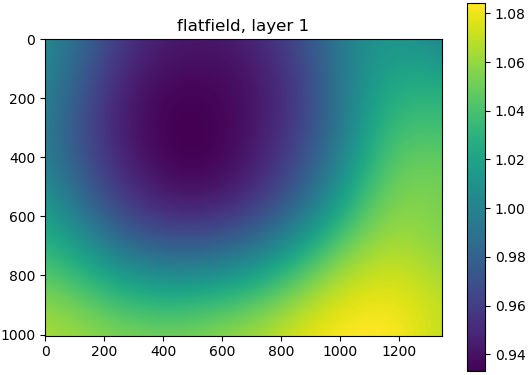
\includegraphics[width=0.3\textwidth]{images/results/flatfield_layers/flatfield_layer_1}
\includegraphics[width=0.3\textwidth]{images/results/flatfield_layers/flatfield_layer_5}
\includegraphics[width=0.3\textwidth]{images/results/flatfield_layers/flatfield_layer_9}
\includegraphics[width=0.3\textwidth]{images/results/flatfield_layers/flatfield_layer_10}
\includegraphics[width=0.3\textwidth]{images/results/flatfield_layers/flatfield_layer_14}
\includegraphics[width=0.3\textwidth]{images/results/flatfield_layers/flatfield_layer_18}
\includegraphics[width=0.3\textwidth]{images/results/flatfield_layers/flatfield_layer_19}
\includegraphics[width=0.3\textwidth]{images/results/flatfield_layers/flatfield_layer_22}
\includegraphics[width=0.3\textwidth]{images/results/flatfield_layers/flatfield_layer_25}
\includegraphics[width=0.3\textwidth]{images/results/flatfield_layers/flatfield_layer_26}
\includegraphics[width=0.3\textwidth]{images/results/flatfield_layers/flatfield_layer_29}
\includegraphics[width=0.3\textwidth]{images/results/flatfield_layers/flatfield_layer_32}
\includegraphics[width=0.3\textwidth]{images/results/flatfield_layers/flatfield_layer_33}
\includegraphics[width=0.3\textwidth]{images/results/flatfield_layers/flatfield_layer_34}
\includegraphics[width=0.3\textwidth]{images/results/flatfield_layers/flatfield_layer_35}
\caption{\footnotesize Layers of the flatfield image, $F_{ijm}$, for $m=$1, 5, 9, 10, 14, 18, 29, 22, 25, 26, 29, 32, 33, 34, and 35 from upper left to lower right, respectively.}
\label{fig:flatfield_image_layers}
\end{figure}

\begin{figure}[!ht]
\centering
\includegraphics[width=0.90\textwidth]{images/results/flatfield_pixel_intensities}
\caption{\footnotesize Maximum, minimum, 5th and 95th percentile, and standard deviation of the flatfield correction factors measured in each layer computed using the full images (red lines and green shading) and only the central 64\% of interest (blue lines and orange shading).}
\label{fig:flatfield_pixel_intensities}
\end{figure} 

%%%%%%%%%%% Reduction in illumination variation subsection
\subsection{Reduction in illumination variation}
\label{ssec:reduction_in_illumination_variation}

The effects of applying the flatfield corrections are measured using an independent set of 22,692 initial HPF images from the same 46 Vectra 3.0 melanoma samples. The images in the test set are masked and selected identically to those used to produce the flatfield, to characterize the impact on the illumination of the fluorescent tissue alone. The number of images stacked in each layer of the test set is shown in \reffig{fig:test_set_n_images_stacked}; removing images on the edges of the tissue reduces the initial number of HPFs from 22,692 to 19,045, and 11,520 images are selected to be stacked on average.

\begin{figure}[!ht]
\centering
\includegraphics[width=0.80\textwidth]{images/results/n_images_stacked_per_layer_test_set}
\caption{\footnotesize Number of images $N_{m}$ selected to be stacked in each layer for the test set of 22,692 independent initial HPFs from 46 Vectra 3.0 samples.}
\label{fig:test_set_n_images_stacked}
\end{figure} 

The masked images are stacked, averaged, and smoothed, using the same procedure described in \refsec{sec:measuring_flatfield_corrections} to produce a mean image $\Iota$ and a smoothed mean image $G$. The smoothed mean image is shown in \reffig{fig:uncorrected_mean_image_layers} for the first, middle, and last layer in each broadband filter region. The patterns in the test image set's $G$ are very similar to those observed in the flatfield image layers shown in \reffig{fig:flatfield_image_layers}. 

\begin{figure}[!ht]
\centering
\includegraphics[width=0.3\textwidth]{images/results/smoothed_mean_image_layers/smoothed_mean_image_layer_1}
\includegraphics[width=0.3\textwidth]{images/results/smoothed_mean_image_layers/smoothed_mean_image_layer_5}
\includegraphics[width=0.3\textwidth]{images/results/smoothed_mean_image_layers/smoothed_mean_image_layer_9}
\includegraphics[width=0.3\textwidth]{images/results/smoothed_mean_image_layers/smoothed_mean_image_layer_10}
\includegraphics[width=0.3\textwidth]{images/results/smoothed_mean_image_layers/smoothed_mean_image_layer_14}
\includegraphics[width=0.3\textwidth]{images/results/smoothed_mean_image_layers/smoothed_mean_image_layer_18}
\includegraphics[width=0.3\textwidth]{images/results/smoothed_mean_image_layers/smoothed_mean_image_layer_19}
\includegraphics[width=0.3\textwidth]{images/results/smoothed_mean_image_layers/smoothed_mean_image_layer_22}
\includegraphics[width=0.3\textwidth]{images/results/smoothed_mean_image_layers/smoothed_mean_image_layer_25}
\includegraphics[width=0.3\textwidth]{images/results/smoothed_mean_image_layers/smoothed_mean_image_layer_26}
\includegraphics[width=0.3\textwidth]{images/results/smoothed_mean_image_layers/smoothed_mean_image_layer_29}
\includegraphics[width=0.3\textwidth]{images/results/smoothed_mean_image_layers/smoothed_mean_image_layer_32}
\includegraphics[width=0.3\textwidth]{images/results/smoothed_mean_image_layers/smoothed_mean_image_layer_33}
\includegraphics[width=0.3\textwidth]{images/results/smoothed_mean_image_layers/smoothed_mean_image_layer_34}
\includegraphics[width=0.3\textwidth]{images/results/smoothed_mean_image_layers/smoothed_mean_image_layer_35}
\caption{\footnotesize Layers of the test dataset smoothed mean image, $G_{ijm}$, for $m=$1, 5, 9, 10, 14, 18, 29, 22, 25, 26, 29, 32, 33, 34, and 35 from upper left to lower right, respectively.}
\label{fig:uncorrected_mean_image_layers}
\end{figure}

The flatfield corrections are applied by dividing the mean image by the flatfield image, pixel-by-pixel, to produce a corrected mean image $\Iota'_{ijm}=\Iota_{ijm}/F_{ijm}$. This layers of this corrected mean image are then smoothed with a $100$ pixel-wide Gaussian filter to produce a smoothed corrected mean image $C_{ijm}$. This $C$ image is shown in \reffig{fig:corrected_smoothed_mean_image_layers_same_scale} for the first, middle, and last layers in each broadband filter region, with the $z$-axis scales identical to those in \reffig{fig:uncorrected_mean_image_layers} to show the bulk effects of applying the flatfield corrections.

\begin{figure}[!ht]
\centering
\includegraphics[width=0.3\textwidth]{images/results/smoothed_corrected_mean_image_layers/smoothed_corrected_mean_image_layer_1_same_scale}
\includegraphics[width=0.3\textwidth]{images/results/smoothed_corrected_mean_image_layers/smoothed_corrected_mean_image_layer_5_same_scale}
\includegraphics[width=0.3\textwidth]{images/results/smoothed_corrected_mean_image_layers/smoothed_corrected_mean_image_layer_9_same_scale}
\includegraphics[width=0.3\textwidth]{images/results/smoothed_corrected_mean_image_layers/smoothed_corrected_mean_image_layer_10_same_scale}
\includegraphics[width=0.3\textwidth]{images/results/smoothed_corrected_mean_image_layers/smoothed_corrected_mean_image_layer_14_same_scale}
\includegraphics[width=0.3\textwidth]{images/results/smoothed_corrected_mean_image_layers/smoothed_corrected_mean_image_layer_18_same_scale}
\includegraphics[width=0.3\textwidth]{images/results/smoothed_corrected_mean_image_layers/smoothed_corrected_mean_image_layer_19_same_scale}
\includegraphics[width=0.3\textwidth]{images/results/smoothed_corrected_mean_image_layers/smoothed_corrected_mean_image_layer_22_same_scale}
\includegraphics[width=0.3\textwidth]{images/results/smoothed_corrected_mean_image_layers/smoothed_corrected_mean_image_layer_25_same_scale}
\includegraphics[width=0.3\textwidth]{images/results/smoothed_corrected_mean_image_layers/smoothed_corrected_mean_image_layer_26_same_scale}
\includegraphics[width=0.3\textwidth]{images/results/smoothed_corrected_mean_image_layers/smoothed_corrected_mean_image_layer_29_same_scale}
\includegraphics[width=0.3\textwidth]{images/results/smoothed_corrected_mean_image_layers/smoothed_corrected_mean_image_layer_32_same_scale}
\includegraphics[width=0.3\textwidth]{images/results/smoothed_corrected_mean_image_layers/smoothed_corrected_mean_image_layer_33_same_scale}
\includegraphics[width=0.3\textwidth]{images/results/smoothed_corrected_mean_image_layers/smoothed_corrected_mean_image_layer_34_same_scale}
\includegraphics[width=0.3\textwidth]{images/results/smoothed_corrected_mean_image_layers/smoothed_corrected_mean_image_layer_35_same_scale}
\caption{\footnotesize Layers of the test dataset smoothed corrected mean image, $C_{ijm}$, for $m=$1, 5, 9, 10, 14, 18, 29, 22, 25, 26, 29, 32, 33, 34, and 35 from upper left to lower right, respectively. The scales on these images are identical to those in \reffig{fig:uncorrected_mean_image_layers} to show the overall effects.}
\label{fig:corrected_smoothed_mean_image_layers_same_scale}
\end{figure}

The flatfield corrections are, again, most relevant in the central 64\% of HPFs that are used for pathology analysis. \reffig{fig:illumination_variation_reduction} shows the minimum, maximum, 5th and 95th percentile, and standard deviation of the pixel intensity relative to the layer mean for the central region of the uncorrected smoothed mean image $G$ and the corrected smoothed mean image $C$. Applying the flatfield corrections greatly reduces the illumination variation observed in the central regions of HPFs: the average spread in the 5th to 95th percentile of the mean-normalized pixel intensity decreases from 11.2\% to 1.2\% on average over all layers, and the standard deviation of the mean-normalized pixel intensity decreases from 3.64\% to 0.37\% on average over all layers.

\begin{figure}[!ht]
\centering
\includegraphics[width=0.90\textwidth]{images/results/illumination_variation_reduction}
\caption{\footnotesize Maximum, minimum, 5th and 95th percentile, and standard deviation of the pixel intensity flux relative to the layer mean in the central 64\% of the uncorrected smoothed mean image $G$ (red lines and green shading) and the corrected smoothed mean image $C$ (blue lines and orange shading) determined from an independent set of HPFs from 46 samples collected with the Vectra 3.0 microscope.}
\label{fig:illumination_variation_reduction}
\end{figure} 

In addition to reducing the overall amount of illumination variation, applying the flatfielding corrections also greatly reduces the systematic patterns in those variations. \reffig{fig:corrected_smoothed_mean_image_layers} shows the same smoothed corrected mean image $C$ as that in \reffig{fig:corrected_smoothed_mean_image_layers_same_scale}, but with the image scales stretched from maximum to minimum. The observed patterns are distinct from those observed for the flatfield corrections (in \reffig{fig:flatfield_image_layers}) or for the uncorrected smoothed mean image (in \reffig{fig:uncorrected_mean_image_layers}), and they show less correlation between different layers contributing to the same broadband filter region.

\begin{figure}[!ht]
\centering
\includegraphics[width=0.3\textwidth]{images/results/smoothed_corrected_mean_image_layers/smoothed_corrected_mean_image_layer_1}
\includegraphics[width=0.3\textwidth]{images/results/smoothed_corrected_mean_image_layers/smoothed_corrected_mean_image_layer_5}
\includegraphics[width=0.3\textwidth]{images/results/smoothed_corrected_mean_image_layers/smoothed_corrected_mean_image_layer_9}
\includegraphics[width=0.3\textwidth]{images/results/smoothed_corrected_mean_image_layers/smoothed_corrected_mean_image_layer_10}
\includegraphics[width=0.3\textwidth]{images/results/smoothed_corrected_mean_image_layers/smoothed_corrected_mean_image_layer_14}
\includegraphics[width=0.3\textwidth]{images/results/smoothed_corrected_mean_image_layers/smoothed_corrected_mean_image_layer_18}
\includegraphics[width=0.3\textwidth]{images/results/smoothed_corrected_mean_image_layers/smoothed_corrected_mean_image_layer_19}
\includegraphics[width=0.3\textwidth]{images/results/smoothed_corrected_mean_image_layers/smoothed_corrected_mean_image_layer_22}
\includegraphics[width=0.3\textwidth]{images/results/smoothed_corrected_mean_image_layers/smoothed_corrected_mean_image_layer_25}
\includegraphics[width=0.3\textwidth]{images/results/smoothed_corrected_mean_image_layers/smoothed_corrected_mean_image_layer_26}
\includegraphics[width=0.3\textwidth]{images/results/smoothed_corrected_mean_image_layers/smoothed_corrected_mean_image_layer_29}
\includegraphics[width=0.3\textwidth]{images/results/smoothed_corrected_mean_image_layers/smoothed_corrected_mean_image_layer_32}
\includegraphics[width=0.3\textwidth]{images/results/smoothed_corrected_mean_image_layers/smoothed_corrected_mean_image_layer_33}
\includegraphics[width=0.3\textwidth]{images/results/smoothed_corrected_mean_image_layers/smoothed_corrected_mean_image_layer_34}
\includegraphics[width=0.3\textwidth]{images/results/smoothed_corrected_mean_image_layers/smoothed_corrected_mean_image_layer_35}
\caption{\footnotesize Layers of the test dataset smoothed corrected mean image, $C_{ijm}$, for $m=$1, 5, 9, 10, 14, 18, 29, 22, 25, 26, 29, 32, 33, 34, and 35 from upper left to lower right, respectively. The image layers shown here are identical to those in \reffig{fig:corrected_smoothed_mean_image_layers_same_scale}, but with the scales stretched from minimum to maximum to show the patterns more than the overall effects.}
\label{fig:corrected_smoothed_mean_image_layers}
\end{figure}

%%%%%%%%%%% Impact of masking subsection
\subsection{Impact of masking}
\label{ssec:impact_of_masking}

To illustrate the improvement provided by masking and selecting images for tissue content, the flatfield corrections were also measured and applied using the same sets of images as above, but with the difference that every image was allowed to contribute all of its pixels instead of discarding any images appearing on the edges of tissue or showing less than 80\% tissue as masked. The flatfield image layers computed using the unmasked set of images are visually very similar to those shown in \reffig{fig:flatfield_image_layers}, with a few specific differences. \reffig{fig:masked_over_unmasked_flatfield_image_layers} shows the masked flatfield divided by the unmasked flatfield for the first, middle, and last layers contributing to each broadband filter region. The major difference is that the unmasked flatfield corrections tend to be larger in scale overall, especially in the lower right hand corners of the images. The maximum and minimum correction factors in the unmasked case are 1.22 and 0.89, respectively, for the entire images, and 1.14 and 0.90, respectively, for the central regions of the images.

\begin{figure}[!ht]
\centering
\includegraphics[width=0.3\textwidth]{images/results/masked_over_unmasked_flatfield_image_layers/masked_over_unmasked_flatfield_image_layer_1}
\includegraphics[width=0.3\textwidth]{images/results/masked_over_unmasked_flatfield_image_layers/masked_over_unmasked_flatfield_image_layer_5}
\includegraphics[width=0.3\textwidth]{images/results/masked_over_unmasked_flatfield_image_layers/masked_over_unmasked_flatfield_image_layer_9}
\includegraphics[width=0.3\textwidth]{images/results/masked_over_unmasked_flatfield_image_layers/masked_over_unmasked_flatfield_image_layer_10}
\includegraphics[width=0.3\textwidth]{images/results/masked_over_unmasked_flatfield_image_layers/masked_over_unmasked_flatfield_image_layer_14}
\includegraphics[width=0.3\textwidth]{images/results/masked_over_unmasked_flatfield_image_layers/masked_over_unmasked_flatfield_image_layer_18}
\includegraphics[width=0.3\textwidth]{images/results/masked_over_unmasked_flatfield_image_layers/masked_over_unmasked_flatfield_image_layer_19}
\includegraphics[width=0.3\textwidth]{images/results/masked_over_unmasked_flatfield_image_layers/masked_over_unmasked_flatfield_image_layer_22}
\includegraphics[width=0.3\textwidth]{images/results/masked_over_unmasked_flatfield_image_layers/masked_over_unmasked_flatfield_image_layer_25}
\includegraphics[width=0.3\textwidth]{images/results/masked_over_unmasked_flatfield_image_layers/masked_over_unmasked_flatfield_image_layer_26}
\includegraphics[width=0.3\textwidth]{images/results/masked_over_unmasked_flatfield_image_layers/masked_over_unmasked_flatfield_image_layer_29}
\includegraphics[width=0.3\textwidth]{images/results/masked_over_unmasked_flatfield_image_layers/masked_over_unmasked_flatfield_image_layer_32}
\includegraphics[width=0.3\textwidth]{images/results/masked_over_unmasked_flatfield_image_layers/masked_over_unmasked_flatfield_image_layer_33}
\includegraphics[width=0.3\textwidth]{images/results/masked_over_unmasked_flatfield_image_layers/masked_over_unmasked_flatfield_image_layer_34}
\includegraphics[width=0.3\textwidth]{images/results/masked_over_unmasked_flatfield_image_layers/masked_over_unmasked_flatfield_image_layer_35}
\caption{\footnotesize Ratios of masked flatfield correction image layers to unmasked flatfield correction image layers for $m=$1, 5, 9, 10, 14, 18, 29, 22, 25, 26, 29, 32, 33, 34, and 35 from upper left to lower right, respectively.}
\label{fig:masked_over_unmasked_flatfield_image_layers}
\end{figure}

The unmasked flatfield corrections were applied to the unmasked test image set in the same way as described in \refsec{ssec:reduction_in_illumination_variation}. When no masking and image selection was performed, the central region of interest of the test dataset's mean image 5th to 95th percentile of mean-normalized pixel intensity was 12.1\% before correction and 1.5\% after correction on average over all layers, and the standard deviation was 3.95\% before correction and 0.47\% after correction on average over all layers. \reffig{fig:unmasked_illumination_variation_reduction} shows the illumination variation observed in the central image regions before and after application of unmasked flatfield corrections. These reductions in average illumination variation are slightly less than those observed for the case where images are masked and selected for tissue content. 

\begin{figure}[!ht]
\centering
\includegraphics[width=0.90\textwidth]{images/results/unmasked_flatfield_illumination_variation_reduction}
\caption{\footnotesize Maximum, minimum, 5th and 95th percentile, and standard deviation of the pixel intensity flux relative to the layer mean in the central 64\% of the uncorrected smoothed mean image $G$ (red lines and green shading) and the corrected smoothed mean image $C$ (blue lines and orange shading) determined from an independent set of HPFs from 46 samples collected with the Vectra 3.0 microscope without any masking or selection of images for tissue content.}
\label{fig:unmasked_illumination_variation_reduction}
\end{figure} 

The smoothed corrected mean image in the unmasked case is shown in \reffig{fig:unmasked_smoothed_corrected_mean_image_layers} for the first, middle, and last layers contributing to each broadband filter region. Compared to the image layers shown in \reffig{fig:corrected_smoothed_mean_image_layers}, the unmasked case results in slightly more systematic patterns of remaining illumination variation. Also interesting to note is the lower overall values of the average illumination flux in every image layer, due to the inclusion of so much dim background.

\begin{figure}[!ht]
\centering
\includegraphics[width=0.3\textwidth]{images/results/unmasked_smoothed_corrected_mean_image_layers/unmasked_smoothed_corrected_mean_image_layer_1}
\includegraphics[width=0.3\textwidth]{images/results/unmasked_smoothed_corrected_mean_image_layers/unmasked_smoothed_corrected_mean_image_layer_5}
\includegraphics[width=0.3\textwidth]{images/results/unmasked_smoothed_corrected_mean_image_layers/unmasked_smoothed_corrected_mean_image_layer_9}
\includegraphics[width=0.3\textwidth]{images/results/unmasked_smoothed_corrected_mean_image_layers/unmasked_smoothed_corrected_mean_image_layer_10}
\includegraphics[width=0.3\textwidth]{images/results/unmasked_smoothed_corrected_mean_image_layers/unmasked_smoothed_corrected_mean_image_layer_14}
\includegraphics[width=0.3\textwidth]{images/results/unmasked_smoothed_corrected_mean_image_layers/unmasked_smoothed_corrected_mean_image_layer_18}
\includegraphics[width=0.3\textwidth]{images/results/unmasked_smoothed_corrected_mean_image_layers/unmasked_smoothed_corrected_mean_image_layer_19}
\includegraphics[width=0.3\textwidth]{images/results/unmasked_smoothed_corrected_mean_image_layers/unmasked_smoothed_corrected_mean_image_layer_22}
\includegraphics[width=0.3\textwidth]{images/results/unmasked_smoothed_corrected_mean_image_layers/unmasked_smoothed_corrected_mean_image_layer_25}
\includegraphics[width=0.3\textwidth]{images/results/unmasked_smoothed_corrected_mean_image_layers/unmasked_smoothed_corrected_mean_image_layer_26}
\includegraphics[width=0.3\textwidth]{images/results/unmasked_smoothed_corrected_mean_image_layers/unmasked_smoothed_corrected_mean_image_layer_29}
\includegraphics[width=0.3\textwidth]{images/results/unmasked_smoothed_corrected_mean_image_layers/unmasked_smoothed_corrected_mean_image_layer_32}
\includegraphics[width=0.3\textwidth]{images/results/unmasked_smoothed_corrected_mean_image_layers/unmasked_smoothed_corrected_mean_image_layer_33}
\includegraphics[width=0.3\textwidth]{images/results/unmasked_smoothed_corrected_mean_image_layers/unmasked_smoothed_corrected_mean_image_layer_34}
\includegraphics[width=0.3\textwidth]{images/results/unmasked_smoothed_corrected_mean_image_layers/unmasked_smoothed_corrected_mean_image_layer_35}
\caption{\footnotesize Layers of the unmasked test dataset's smoothed corrected mean image for $m=$1, 5, 9, 10, 14, 18, 29, 22, 25, 26, 29, 32, 33, 34, and 35 from upper left to lower right, respectively.}
\label{fig:unmasked_smoothed_corrected_mean_image_layers}
\end{figure}

%%%%%%%%%%%%%%%%%%%%%%%%%%%%%%%%%%%%%%%%%%%%%% SUMMARY SECTION %%%%%%%%%%%%%%%%%%%%%%%%%%%%%%%%%%%%%%%%%%%%%%
\section{Summary}
\label{sec:summary}

The Astropath group has developed a method for correcting systematic variations in the illumination of multiplexed microscope HPF images. The method is optimized for application to the fluorescent tissue only, and the measured corrections are minimally biased to illumination variation observed in the background of the images. A set of 45,384 total HPFs from 46 slides of melanoma tissue imaged using the Vectra 3.0 digital microscope was split into two random groups for independently measuring and testing application of the corrections. The average variation in each layer's mean-normalized 5th to 95th percentile flux decreased from 11.2\% to 1.2\% upon application of the measured corrections, and the average variation in the standard deviation of the mean-normalized flux for each layer decreased from 3.64\% to 0.37\%. The systematic patterns in illumination were also reduced to being more random. Procedures used to mask background out of images were shown to slightly improve the reduction in illumination variation over identical methods based on entire images rather than tissue-containing regions.

%%%%%%%%%%%%%%%%%%%%%%%%%%%%%%%%%%%%%%%%%%%%%%% BIBLIOGRAPHY %%%%%%%%%%%%%%%%%%%%%%%%%%%%%%%%%%%%%%%%%%%%%%%%
\clearpage
\bibliography{references}

\end{document}